\chapter{不完美信息扩展型博弈}

虽然本章位置相对靠后，但本章介绍的内容是非合作博弈理论的重要组成部分。本章介绍不完美信息扩展型博弈，这类博弈可以通过具有不完美信息的博弈树进行刻画。通常情况下，参与人并不总是能获取全部与他们选择相关的信息。具有不完美信息的扩展型博弈能够精确地刻画参与人在行动时拥有的信息。对策略信息进行精准建模和分析是博弈论的一大优势。

第10.2节通过一个详细的例子引入信息集这一核心概念。后续章节给出扩展型博弈的一般定义，以及策略和精简策略的定义。这些定义推广了之前在介绍完美信息的扩展型博弈时引入的概念。本质上，只需将“决策节点”替换为“信息集”即可。

第10.6节介绍完美记忆这一概念。它指的是参与人总是记得他之前知道的信息或采取的行动。它是约束的是参与人信息集的结构的条件，而不是对博弈的解读。第10.8节介绍Kuhn(1953)的重要定理（定理10.4）。该定理表明在具有完美记忆的博弈中，参与人可以用行为策略（behavior strategy）替代任何混合策略。行为策略是指参与人在每个信息集上局部地对他的行动进行随机化。相比之下，混合策略则是首先在博弈开始时全局地选择一个纯策略，随后参与人在整个博弈过程中将其作为行动计划来执行。行为策略比混合策略简单得多，这一点我们后续将详细说明。第10.9节，我们将介绍“蒙提·霍尔”问题的博弈论变体问题，并给出最优混合策略和行为策略（该问题的结果与标准的统计版本的结果相反）。

最后的10.10节讨论子博弈和子博弈完美均衡。

\section{预备知识和学习目标}

本章的预备知识包括第4章和第6章。学习本章后，你应该能够:

\begin{itemize}
\item 解释扩展型博弈和信息集的概念；
\item 描述扩展型博弈的纯策略和精简纯策略，以及博弈相应的策略形式和精简策略型；
\item 定义完美记忆的概念，并判断给定博弈是否满足这一条件；
\item 解释行为策略和混合策略的区别，并阐述库恩定理（定理10.4）；
\item 根据不完全信息博弈的描述构建扩展型博弈，如练习~\ref{exer:10.4}；
\item 找出简单扩展型博弈的所有均衡，并将这些均衡中的混合策略表示为行为策略；
\item 解释子博弈和子博弈完美均衡的概念，以及该概念如何推广了逆向归纳法，并且区别在何处。理解当博弈树存在不完全信息时，像逆向归纳法那样每次只选择单个行动的方法将不再适用。
\end{itemize}


\section{信息集}

我们来考虑如下情景：一家小型初创企业（参与人$\mathrm{II}$）宣布将推出一项关键新技术，大型软件公司（参与人$\mathrm{I}$）由此面临的相应局面。大型公司拥有庞大的研发部门。众所周知的是，他们的研究人员在进行各种各样的创新研究。然而只有大型公司自己确切知道他们是否在与小型公司新技术类似的产品上取得了进展。初创公司认为，大型公司有50\%的可能性已经具备了生产强有力竞争产品的基础。简洁起见，当大型公司有能力生产强有力的竞争产品时，我们称大型公司是强势的，否则称其弱势的。

大型公司在初创公司宣布后有两个选择：它可以宣布也将推出竞争产品，或者放弃该产品的市场；并且它肯定会根据其自身是强势的还是弱势的的私人信息来做出选择。如果大型公司宣布推出产品，那么初创公司有两个选择：它可以与大型公司协商让它收购自己，或者保持独立并推出自己的产品。初创公司无法获取大型公司研发状况的私人信息，然而它能观察到大型公司是否宣布推出自己的产品，并试图从该宣布中推断大型公司是强势的还是弱势的。

\begin{figure}[htbp]
\centering
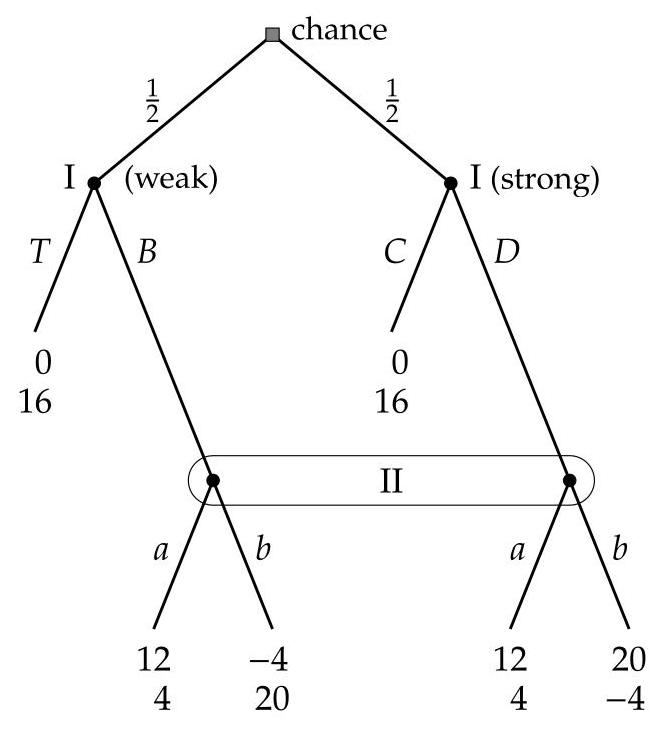
\includegraphics[width=0.3\textwidth]{images/ch10-fig01.jpg}
\caption{参与人$\mathrm{II}$的不完全信息博弈，由包含两个具有相同行动 \(a\) 和 \(b\) 的决策节点的信息集表示。和前文一样，在树的叶节点处，上面的收益属于参与人 \(I\)，下面的收益属于参与人$\mathrm{II}$。}
\label{fig:10.1}
\end{figure}

当大型公司是弱势时，初创公司更愿意留在市场而不是被大型公司收购。当大型公司是强势时，情况则相反，初创公司更愿意被收购。

图~\ref{fig:10.1}展示的是一个模拟这种情况的不完全信息博弈树(也被称为扩展型博弈)。从初创公司的角度来看，大型公司是弱势的还是强势的是随机的。我们通过一个初始的随机行动来建模这一情况，并假设两种可能性的概率均为 \(\frac{1}{2}\) 。

当大型公司是弱势时，它可以选择将市场让给初创公司，这里记为行动 \(T\)，参与人$\mathrm{I}$和II的即时收益分别为0和16。它也可以宣布推出竞争产品，用行动 \(B\) 表示，寄希望于初创公司(参与人$\mathrm{II}$)选择行动 \(a\) 将公司出售套现；此时两个参与人的收益分别为12和4。然而，如果参与人$\mathrm{II}$选择行动 \(b\) 决定留在市场，那么它甚至会从增加的知名度中获利，获得收益20，而参与人$\mathrm{I}$的收益为 -4。

相反，当参与人$\mathrm{I}$是强势时，它既可以再次将市场让给参与人$\mathrm{II}$（选择行动 \(C\)，此时的收益组合与之前一样，为0和16），也可以宣布推出自己的产品（选择行动 \(D\) ）。显然，参与人$\mathrm{I}$绝不应该选择行动 \(C\)，但我们仍将其视为一种可能的行动。在强势的参与人$\mathrm{I}$选择行动 \(D\) 之后，如果初创企业出售（选择行动 \(a\) ），那么两个参与人的收益为12和4；如果初创企业继续留在市场（选择行动 \(b\) ），收益为 \({20}\) 和\(- 4\) 。


与具有完美信息的博弈树相比，本模型有一个额外的特点：部分参与人的某些决策节点被椭圆框圈起来。这些椭圆定义了信息集。信息集是一些决策节点的集合，需满足我们稍后将详细描述的特定限制条件。其含义是，当参与者做出行动决策时，依据自身所掌握的信息，无法区分同一信息集内的各个节点。由于参与人在该信息集的全部节点处所拥有的信息完全相同，因此他会在集合内的每一个节点上做出相同的行动选择。在这一问题中，初创企业即参与人$\mathrm{II}$，必须在行动 \(a\) （出售）和行动 \(b\) （留在市场）之间做出选择。这就是参与人$\mathrm{II}$在其信息集下的两项行动选择。该信息集包含两个节点，对应两种不同的博弈历史，而参与者 II 无法区分这两个节点。

由于参与人$\mathrm{II}$在博弈过程中不清楚自己所处的位置，逆向归纳法不再适用。如果参与人$\mathrm{II}$知道参与人$\mathrm{I}$是强势的还是弱势的，那么当参与人 \(\mathrm{I}\) 弱势时，她选择 \(b\) 收益更多；当参与人 \(\mathrm{I}\) 强势时，她选择 \(a\) 收益更多。

参与人$\mathrm{I}$也有信息集，他的每个决策节点就对应一个信息集。每个信息集仅包含一个节点表明参与人对博弈状态有完美的了解。在博弈树中，我们不会画出这些单节点信息集；当一个决策节点没有被椭圆圈起来时，就意味着它是单点信息集。

从博弈树中可以直接看出的一个最优行动是，参与人$\mathrm{I}$强势时选择行动 \(D\) 。参与人$\mathrm{I}$选择 \(C\)的收益为零，而选择 \(D\) 的收益，当参与人$\mathrm{II}$选择 \(a\) 或\(b\)时 ，分别是12或20，这两个值都大于零，所以参与人$\mathrm{I}$无论如何都应该选择 \(D\) 。由此博弈就简化为参与人$\mathrm{I}$只需在行动 \(T\) 和 \(B\) 之间进行选择，参与人$\mathrm{II}$则在\(a\) 和 \(b\) 之间进行选择。


从博弈树中可以看出，两个参与人的任何一个行动组合，都不是针对对方的行动的最优反应。对于参与人$\mathrm{I}$来说，如果参与人$\mathrm{II}$选择 \(b\)，那么行动 \(T\) 更好（因为收益0比 -4 高）。如果参与人$\mathrm{I}$选择 \(T\)，那么参与人$\mathrm{II}$信息集的左节点就不会被触及。在这种情况下，当参与人$\mathrm{II}$在 \(a\) 和 \(b\) 之间进行选择时，她可以确定自己处于其信息集的右节点。因此，她选择 \(a\) 能获得较高的收益4（而选择 \(b\) 时收益为 -4 ）。反过来，如果参与人$\mathrm{II}$选择 \(a\)，那么即使是弱势的参与人$\mathrm{I}$也会选择 \(B\) 而非 \(T\)，因为前者的收益12高于后者的收益0。如果参与人$\mathrm{I}$选择 \(B\)，那么参与人$\mathrm{II}$处于其信息集的左节点或右节点的概率相等。此时，参与人$\mathrm{II}$在比较 \(a\) 和 \(b\) 时必须使用期望效用。显然，行动 \(a\) 会给她带来收益4，而行动 \(b\) 会给她带来期望效用 \(\frac{1}{2} \cdot  {20} + \frac{1}{2} \cdot  \left( {-4}\right)  = 8\) 。该期望效用超过了行动 \(a\) 的收益。也就是说，针对 \(B\)，参与人$\mathrm{II}$选择 \(b\) 会更好。现在我们又回到了原点:参与人的最优反应行动序列为 \(b \rightarrow  T \rightarrow  a \rightarrow  B \rightarrow  b\)，因此不存在能够构成均衡的确定性行动。

\begin{figure}[htbp]
\centering
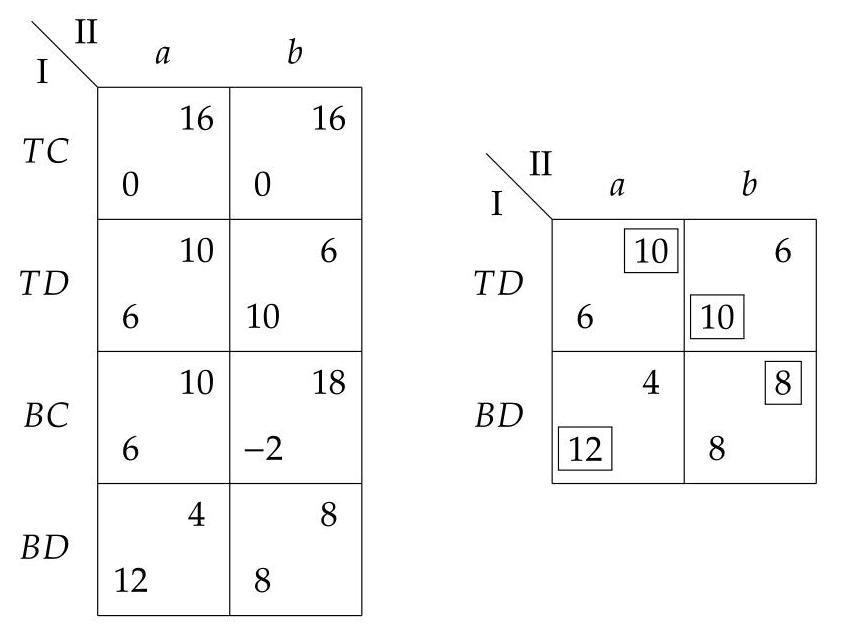
\includegraphics[width=0.6\textwidth]{images/ch10-fig02.jpg}
\caption{左:图~\ref{fig:10.1}中博弈的策略形式。右:消除严格被占优策略 \(2 \times 2\) 和 \({BC}\) 后得到的博弈，方框标注了最优反应效用。}
\label{fig:10.2}
\end{figure}

因为每位参与者都只有两个关键行动，图~\ref{fig:10.1} 所示的博弈仅依靠行动就可以完成分析（本节末尾将给出该分析过程）。但一般而言，借鉴完全信息博弈树中已经定义过的博弈的策略型式表述是有帮助的。原因在于策略型式需要系统考察参与者的策略，以及均衡概念也是基于策略而非行动来定义的。

图~\ref{fig:10.2}中的左表给出了图~\ref{fig:10.1}中博弈的策略形式。与具有完美信息的博弈树一样，参与人的策略为该参与人的每个决策节点定义了一个行动。然而，不同之处在于，对于属于一个信息集的所有决策节点，这样的行动只定义一次。因为根据定义，无论参与人在信息集中的哪个位置，该行动的选择都是相同的。在图~\ref{fig:10.1}中，这意味着参与人$\mathrm{II}$只有两种行动，即她在信息集处的两种行动 \(a\) 和 \(b\) 。因为参与人$\mathrm{II}$只有一个信息集，所以她的策略与她的行动相同。参与人$\mathrm{I}$有两个信息集，所以参与人$\mathrm{I}$的一个策略是一对行动，一个是第一个信息集的行动，另一个是第二个信息集的行动。这些行动对是 \({TC},{TD},{BC}\) 和 \({BD}\) 。

参与人$\mathrm{I}$的四种策略对应于图~\ref{fig:10.2}左图中的行，而参与人$\mathrm{II}$的策略 \(a\) 和 \(b\) 对应于列。该表中的每个单元格给出了根据叶节点的效用和机会概率计算出的期望效用。例如，策略对 (BC, a) 给参与人$\mathrm{I}$带来期望效用 \(\frac{1}{2} \cdot  {12} + \frac{1}{2} \cdot  0 = 6\)，给参与人$\mathrm{II}$带来效用 \(\frac{1}{2} \cdot  4 + \frac{1}{2} \cdot  {16} = {10}\) 。这些期望来自随机行动，根据图~\ref{fig:10.1}，这两种随机行动的概率都是 \(\frac{1}{2}\) 。当随机行动向左时，策略对 (BC, a) 意味着博弈的进行遵循行动 \(B\)，然后是行动 \(a\)，并到达给参与人$\mathrm{I}$、II带来效用12、4的叶节点。当随机行动向右时，策略对 (BC, a) 意味着行动 \(C\) 直接到达给参与人$\mathrm{I}$、II带来效用0、16的叶节点。

图~\ref{fig:10.2}左侧的 \(4 \times  2\) 博弈有两个严格被占优策略，即 \({TC}\)，它被 \({TD}\) 严格占优，以及 \({BC}\)，它被 \({BD}\) 严格占优。这与我们之前的观察一致：对于参与人$\mathrm{I}$来说，无论参与人$\mathrm{II}$采取什么行动，行动 \(C\) 总是比行动 \(D\) 差。然而，我们必须谨慎地得出“较差的行动总是会导致严格被占优策略”这一的结论（举例来说，用较差的行动 \(C\) 替换策略 \({TD}\) 中给定的 \(D\)，就会得到被占优策略 \({TC}\)  ）。即使较差的行动 \(C\) 带来的收益严格低于给定行动\(D\)，也必须保证可供选择 \(C\)和\(D\) 这两个行动的决策节点，总能够以正概率到达。只有满足该条件，两种策略的期望收益才一定会出现差异。在本例中该条件成立，因为参与人$\mathrm{I}$选择行动 \(C\) 和 \(D\) 的决策点是通过一个随机行动到达的。作为比较，倘若将该随机行动改为由第三个参与人做出行动，那么一旦第三个参与人不选择向右行动，$C$ 和 $D$ 之间的抉择就不会对参与人$\mathrm{I}$的收益产生任何影响。因此，在这种情况下，我们只能得出 \({TD}\) 弱占优 \({TC}\) 的结论。简而言之，尽管仔细分析博弈树可能会立即剔除部分策略，但考察博弈的策略形式更为稳妥。

剔除严格被占优策略 \({TC}\) 和 \({BC}\) 后，我们得到图~\ref{fig:10.2}右侧的 \(2 \times  2\) 博弈。在这个博弈中，每个参与人有两种策略，这对应于我们之前讨论的两种行动。方框圈出的是最优反应收益，并且表明这个博弈没有纯策略均衡。

这个博弈存在混合策略均衡，可按照常规方法求解。参与人$\mathrm{I}$以相等的概率 \(\frac{1}{2}\) 在 \({TD}\) 和 \({BD}\) 之间随机选择，使得参与人$\mathrm{II}$选择 \(a\) 和 \(b\) 的期望效用均为7。参与人$\mathrm{II}$以概率 \(\frac{1}{4}\) 选择 \(a\)，以概率 \(\frac{3}{4}\) 选择 \(b\)，使得参与人$\mathrm{I}$选择 \(T\) 和 \(B\) 的期望效用均为 \(\frac{36}{4} = 9\) 。

图~\ref{fig:10.1}对应的是两家企业竞争博弈，如果把它看作扑克牌游戏的一个简化版本时，我们会更熟悉。我们可以设想：参与人$\mathrm{I}$以相等的概率拿到一手弱牌或强牌。参与人$\mathrm{I}$知道自己的牌是弱还是强（在真正的扑克游戏中，参与人$\mathrm{I}$知道自己的牌，但不一定知道它比参与人$\mathrm{II}$的牌好还是差）。然后，参与人$\mathrm{I}$可以选择“弃牌”（行动 \(T\) 和 \(C\) ），或者“加注”（行动 \(B\) 和 \(D\) ）。反过来，参与人$\mathrm{II}$可以选择“放弃”（行动a）或“跟注”（行动b）。弃牌和放弃行动会产生固定结果。在这一结果中，参与人获得的收益与他们手中的牌无关。只有加注和跟注的行动组合，对应于策略组合(BD，b)，才会让参与人手中的牌影响最终收益，如图~\ref{fig:10.1}所示（在策略形式中，受随机行动的影响，不同的策略组合会带来不同的收益）。

如果参与人$\mathrm{I}$持有弱牌并决定加注（行动 \(B\) ），他是在虚张声势，即假装他持有强牌，因为参与人$\mathrm{II}$并不知道他的牌是强是弱。然而，虚张声势的目的不仅是让参与人$\mathrm{II}$弃牌。正如前文分析的，实际上，如果参与人$\mathrm{I}$一直虚张声势，参与人$\mathrm{II}$不会弃牌（行动 \(a\) ）。虚张声势的一个主要效果是让参与人$\mathrm{II}$不确定参与人$\mathrm{I}$持有的是强牌还是弱牌。对参与人$\mathrm{I}$来说，最好的结果是参与人$\mathrm{II}$遇到参与人$\mathrm{I}$的强牌（行动 \(D\) 和 \(b\) ），此时参与人$\mathrm{I}$带来获得最大收益。如果参与人$\mathrm{I}$仅在持有强牌时加注，那么参与人$\mathrm{II}$宁愿弃牌，这对参与人$\mathrm{I}$是不利的。综上所述，正如前文推导过的，不存在确定性的行动组合能构成均衡，借助在扑克牌博弈的视角，可以非常直观地解释这一点。

作为本例讨论的收尾，我们可以直接通过博弈树推导出达到均衡所需要的行动$T$和$B$以及行动$a$和$b$的概率。即使不构建策略形式，我们也已经看到，对这些行动的任何确定性选择都无法得到均衡。因此两位参与人都会采取随机行动，并且各个可选行动给他们带来的期望收益必须是无差异的。对于参与人$\mathrm{I}$来说，这种无差异条件很容易求解：如果他需要在 \(T\) 和 \(B\) 之间做出选择，那么选择 \(T\) 他能获得确定的收益0，所以只有当 \(B\) 的期望效用也为0时，无差异条件才会得到满足。如果参与人$\mathrm{II}$分别以概率 \(1 - q\) 和 \(q\) 选择 \(a\) 和 \(b\)，那么参与人 \(\mathrm{I}\) 的期望效用是 \({12}\left( {1 - q}\right)  - {4q}\)，因此方程 \(0 = {12}\left( {1 - q}\right)  - {4q} = {12} - {16q}\) 得出 \(q = \frac{3}{4}\) 。

相应地，参与人$\mathrm{II}$想要选择随机行动，必须对她的行动 \(a\) 和 \(b\) 无差异。这里的情况稍微复杂一些，因为参与人$\mathrm{II}$的期望效用取决于她在信息集中处于左节点还是右节点的概率。当我们假设参与人$\mathrm{I}$确定地选择 \(D\) 时，那么参与人$\mathrm{II}$处于右节点的概率是 \(\frac{1}{2}\)，而处于左节点的概率是 \(\frac{1}{2} \cdot  p\)，其中 \(p\) 是参与人$\mathrm{I}$选择 \(B\) 的概率。由于行动\(T\) 有非零概率 \(1 - p\) 发生，博弈以概率 \(\frac{1}{2} \cdot  \left( {1 - p}\right)\) 在博弈树的最左叶节点结束，那么参与人$\mathrm{II}$的信息集根本不会被触及。从技术上讲，需要计算的是参与人$\mathrm{II}$处于左节点相对于处于右节点的条件概率。在详细讨论之前，我们可以注意到，根据目前的描述，到达左节点的概率是到达右节点概率的 \(p\) 倍，真正起作用的正是这一对相对权重。参与人$\mathrm{II}$在 \(a\) 和 \(b\) 之间的无差异便可得到如下方程，左右两边分别是 \(a\) 和 \(b\) 的加权收益: \begin{equation}
\label{eq:10.1}
p \cdot  4 + 1 \cdot  4 = p \cdot  {20} + 1 \cdot  \left( {-4}\right).
\end{equation}

该方程可简化为 \({4p} + 4 = {20p} - 4\) 或 \(8 = {16p}\)，即 \(p = \frac{1}{2}\) 。

参与人\(\mathrm{II}\) 位于左、右节点的条件概率计算如下：到达左节点的绝对概率为 \(\frac{1}{2} \cdot  p\)，到达右节点的绝对概率为 \(\frac{1}{2}\) 。位于这两个节点（互斥事件）中任意一个的总概率是这两个概率之和，即 \(\frac{p + 1}{2}\) 。条件概率就是绝对概率除以总概率，因此，到达左节点的条件概率为 \(\frac{p/2}{\left( {p + 1}\right) /2}\) 或 \(\frac{p}{p + 1}\)，到达右节点的条件概率为 \(\frac{1/2}{\left( {p + 1}\right) /2}\) 或 \(\frac{1}{p + 1}\) 。在 (\ref{eq:10.1}) 中使用这些条件概率替代原先的“权重”，意味着将方程 (\ref{eq:10.1}) 的两边同时除以 \(p + 1\) 。这不会改变该方程的解，因此我们之前的推导过程完全成立（只要到达该信息集的总概率不为零）。

我们再次从博弈树的角度来解释均衡概率 \(p = \frac{1}{2}\) 和 \(q = \frac{3}{4}\) :参与人\(\mathrm{I}\) 以概率 \(\frac{1}{2}\) 选择 \(B\)，并确定地选择 \(D\)，使得参与人\(\mathrm{II}\) 位于其信息集左节点的概率是位于右节点的一半。因此，到达左节点和右节点的条件概率分别为 \(\frac{1}{3}\) 和 \(\frac{2}{3}\) （即\(\left. \frac{1}{4}\right.\) 和 \(\frac{1}{2}\) 分别除以到达该信息集的总概率 \(\frac{3}{4}\) ）。正式在该条件下，参与人\(\mathrm{II}\) 对行动 \(a\) 和 \(b\) 无差异：此时参与人\(\mathrm{II}\) 选择行动 \(a\) 的条件期望效用显然为 4，选择行动 \(b\) 的条件期望效用为 \(\frac{1}{3} \cdot  {20} + \frac{2}{3} \cdot  \left( {-4}\right)  = \frac{12}{3} = 4\) 。计算参与人\(\mathrm{II}\) 的总体期望效用需要用到绝对概率：她有\(\frac{1}{4}\) 的概率 （左方随机行动，参与人 \(\mathrm{I}\) 选择 \(T\) ）获得效用16，有 \(\frac{3}{4}\)的概率获得上述条件效用4，总体为 \(\frac{1}{4} \cdot  {16} + \frac{3}{4} \cdot  4 = 4 + 3 = 7\) 。对于参与人\(\mathrm{I}\)，前面已经得到其在 \(T\) 和 \(B\) 之间无差异。当随机行动指向左方时，参与人\(\mathrm{I}\) 获得的效用为零。当随机行动指向右方时，参与人\(\mathrm{I}\) 选择 \(D\) 将获得 \(\left( {1 - q}\right)  \cdot  {12} + q \cdot  {20} = \frac{1}{4} \cdot  {12} + \frac{3}{4} \cdot  {20} = {18}\) 。参与人 \(I\) 的总期望效用为 \(\frac{1}{2} \cdot  0 + \frac{1}{2} \cdot  {18} = 9\) 。

\section{扩展型博弈}

在本节中，我们给出扩展型博弈的一般定义。扩展型博弈也被称为扩展形式的博弈，或具有不完美信息的博弈树。

与第 4 章中考虑的具有完美信息的博弈树类似，扩展型博弈的基本结构是一棵树。和前文介绍的一样，它有三种类型的节点：终端节点，也称为叶节点，为每个参与人提供一个效用；非终端节点中的机会节点（通常画成正方形），下一个节点根据树中指定的给定的概率随机选出；以及非终端节点中的决策节点，这些节点属于特定的参与人。从每个决策节点发出的边都标有选择或行动的名称，这些名称能唯一地标识相应的边。

决策节点被划分为信息集。划分意味着每个决策节点恰好属于一个信息集，且没有信息集为空。在绘制扩展型博弈时，信息集用包含节点的椭圆表示（除非信息集仅包含一个节点）；也有文献会用一条虚线连接信息集中的节点来表示信息集。

信息集的含义是，在博弈过程中，参与人只被告知自己处于某个信息集中的某个节点，但不知道具体是哪个节点。因此，信息集必须满足一些条件：在一个信息集中，所有决策节点都属于同一个参与人；该集合中的所有决策节点具有相同数量的出边；并且信息集中每个节点的行动集合（由出边上的标签给出）是相同的。例如，在图~\ref{fig:10.1}中，参与人$\mathrm{II}$的信息集有两个行动， \(a\) 和 \(b\) 。当参与人到达一个信息集时，他选择一个行动，根据定义，无论他在信息集中的哪个位置，这个行动都是相同的。

如果每个信息集都是单点集（仅包含一个节点；前文提到，我们通常不绘制这些单点集），那么这些条件显然是满足的。如果所有信息集都是单元素集，那么该博弈具有完美信息，信息集也可以省略。这就得到了前问所讨论的具有完美信息的博弈树。只有对于包含两个或更多节点的信息集，上述约束条件才会发挥实际作用。

\begin{figure}[htbp]
\centering
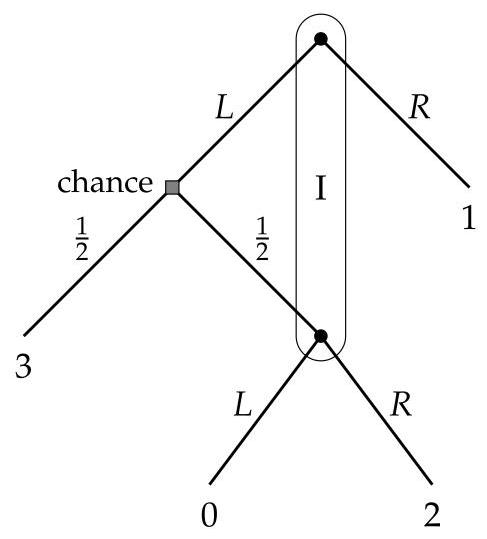
\includegraphics[width=0.3\textwidth]{images/ch10-fig03.jpg}
\caption{一个信息集中两个节点共享一条路径的博弈，这在扩展型博弈中通常是不允许的。}
\label{fig:10.3}
\end{figure}

除了上述条件外，我们还将对信息集的结构施加额外的约束。其中第一个约束是，信息集中的任意两个节点不能位于同一条路径上，参见图~\ref{fig:10.3}中的示例。该图展示的单人博弈中，参与人 \(\mathrm{I}\) 有两个决策节点，它们属于一个具有两个行动 \(L\) 和 \(R\) 的信息集。唯一的其他非终端节点是一个随机行动节点。该博弈满足扩展型博弈的全部前述条件。然而，参与人$\mathrm{I}$的两个决策节点在同一条路径上：第一个节点是根节点，从该节点有一条路径通向第二个节点。很难很好地解释具有这种特征的信息集：因为我们要求在这样的信息集中，例如行动 \(L\)，无论身处集合中的哪一个节点，都必须是同一个行动。然而，在图~\ref{fig:10.3}中，参与人$\mathrm{I}$采取行动 \(L\) 意味着什么呢？这肯定意味着从根节点向左移动，但如果之后随机行动向右移动，使得参与人$\mathrm{I}$可以再次移动，他是否必须再次选择行动 \(L\) 呢？

图~\ref{fig:10.3}中信息集的问题在于，根据信息集的含义，当参与人$\mathrm{I}$需要在 \(L\) 和 \(R\) 之间进行选择时，他必须忘记自己是否采取过行动，甚至不清楚他是否被允许再次行动。信息集可以表示参与人忘记了他之前知道或做过的事情。在这种情况下，我们称参与人具有不完美记忆。然而，具有不完美记忆的参与人不符合我们对“理性”参与人的定义。此外，如果信息集中的一个节点是另一个节点的后代节点，那么参与人究竟可以行动多少次也无法确定。因此，我们将假设所有参与人都具有完美记忆，其严格定义与详细讨论放在下文的10.6节中。具体来说，我们将推导出完美记忆意味着信息集中的任意两个节点在博弈树中不会在同一条路径上(见下文的命题10.2)。由此图~\ref{fig:10.3}这样的情况就会被排除。

综上，我们对不完全信息博弈树的定义做如下总结：唯一新增的概念就是信息集，它用于刻画参与者无法确定自己处于博弈中哪一节点的信息缺失状态。

\section{扩展型博弈的策略型表达}

扩展型博弈中策略的定义，是对具有完美信息的博弈树中策略定义的推广：参与人的（纯）策略要为参与人的每个信息集都指定一个行动。

要对策略进行正式定义，我们需要引入记号，表示参与人的各个信息集，以及每个信息集下可选择的行动。假设参与人 \(i\) 是扩展型博弈中的一个参与人（例如两人博弈中的参与人\(\mathrm{I}\) 或参与人\(\mathrm{II}\)），我们用 \({H}_{i}\) 表示参与人 \(i\) 全部信息集构成的集合，用\(h\) 表示参与人 \(i\) 的一个特定信息集。对于任意的其中 \(h \in  {H}_{i}\)，我们用 \({C}_{h}\) 表示信息集 \(h\) 下的选择或行动集合。例如，如果 \(h\) 是图~\ref{fig:10.1} 中参与人\(\mathrm{I}\) 的左侧信息集，那么 \({C}_{h} = \{ T,B\}\) 。

参与人 \(i\) 的策略集合 \({\sum }_{i}\) 为\begin{equation}
\label{eq:10.2}
{\sum }_{i} = \bigtimes\limits_{{h \in  {H}_{i}}}{C}_{h},
\end{equation} 即参与人 \(i\) 的选择集 \({C}_{h}\) 的笛卡尔积。 \({\sum }_{i}\) 中的一个元素是一个行动元组（向量）：对于参与人 \(i\) 的每个信息集 \(h\)，从 \({C}_{h}\) 中选取一个行动 \(c\) 。

如果 \(N\) 是参与人集合，例如我们在两人博弈符号中使用的 \(N = \{ \mathrm{I},\mathrm{{II}}\}\)，那么纯策略组合的集合是 \(\bigtimes \limits_{{i \in  N}}{\sum }_{i}\) 。也就是说，一个策略组合为每个参与人指定一个纯策略。

\begin{figure}[htbp]
\centering
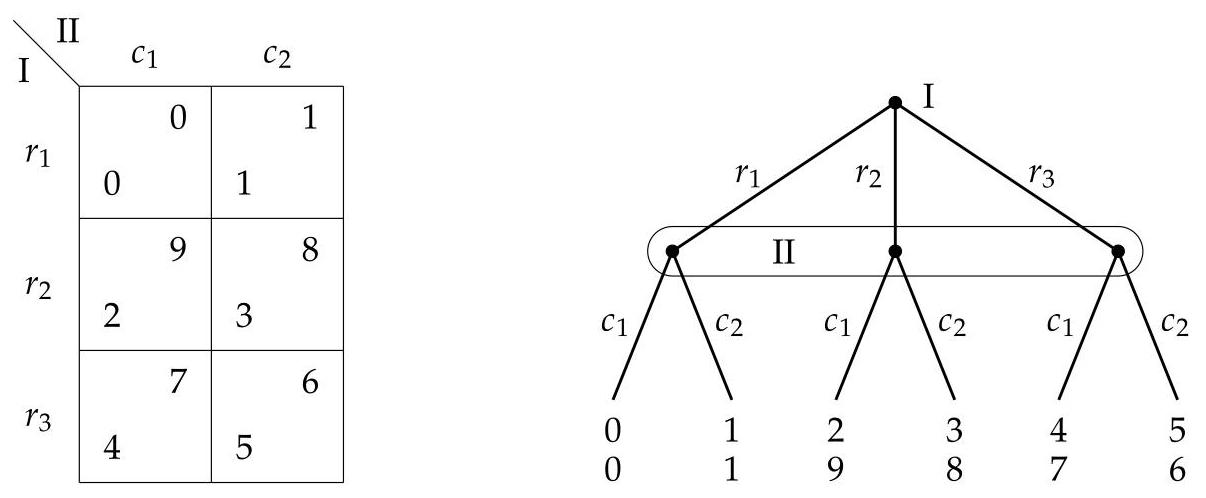
\includegraphics[width=0.9\textwidth]{images/ch10-fig04.jpg}
一个\caption{\(3 \times 2\) 博弈以及一个以该博弈为策略型的扩展型博弈。}
\label{fig:10.4}
\end{figure}

扩展型博弈的策略形式由三部分构成：参与人集合 \(N\) 、每个参与人 \(i\) 的策略集合 \({\sum }_{i}\) 以及每个参与人在每个策略组合下获得的期望效用。如果博弈没有随机行动，那么每个策略组合的收益由参与人使用其策略时到达的博弈树的叶节点确定。如果博弈有随机行动，那么给定一个策略组合可能到达多个叶节点，此时就需要计算期望效用，如图~\ref{fig:10.2} 的例子所示。

借助信息集，可以在扩展型博弈中对同时行动进行建模。这一点是完全信息博弈树无法做到的：在完全信息博弈树中，行动是依次发生的，后行动的参与人能够观察到先行动参与人所选择的行动。

具体而言，给定一个策略型博弈，都存在一个扩展型博弈恰好具有该策略型。以 \(m \times  n\) 博弈为例。哪个参与人先行动并不重要，我们不妨假设是参与人 \(\mathrm{I}\) 先行动。在博弈树的根节点处，他有 \(m\) 个行动 \({r}_{1},{r}_{2},\ldots ,{r}_{m}\)，分别对应于博弈矩阵的 \(m\) 行。参与者\(\mathrm{I}\) 的每一个行动都会通向参与者\(\mathrm{II}\) 的一个决策节点，并且所有这些节点都属于同一个信息集。在该信息集下，参与人\(\mathrm{II}\) 有 \(n\) 个行动 \({c}_{1},{c}_{2},\ldots ,{c}_{n}\)，对应于博弈矩阵的 \(n\) 列。参与人\(\mathrm{II}\) 的每个行动都通向博弈树的一个叶节点。参与者\(\mathrm{I}\)共有$m$个行动，每一种行动之后参与者\(\mathrm{II}\)又有n种行动可选，所以博弈树有 \({mn}\) 个叶节点。假设给定的博弈中，参与人\(\mathrm{I}\) 和参与人\(\mathrm{II}\) 分别选择第 \(i\) 行和第 \(j\) 列时的收益为 \({a}_{ij}\) 和 \({b}_{ij}\)，那么这两个收益在博弈树中通过行动 \({r}_{i}\) 之后接着行动 \({c}_{j}\) 到达的叶节点处，就标注这两个收益。因为每个参与人只有一个信息集，参与人的策略与他的行动是一样的。由此构建的扩展型博弈的策略形式就是原来的 \(m \times  n\) 博弈。博弈矩阵的行用策略标记为 \({r}_{1},\ldots ,{r}_{m}\)，列标记为 \({c}_{1},\ldots ,{c}_{n}\)，这些名称继承扩展式博弈中两位参与人的行动名称。图~\ref{fig:10.4} 给出了一个例子。

\(\Rightarrow\) 练习~\ref{exer:10.1} 要求读者重复上述推导过程，但改为令参与人 \(\mathrm{II}\)先行动，参与人\(\mathrm{I}\)后行动。

\section{精简策略}

考虑图~\ref{fig:10.5}中的扩展型博弈。参与人$\mathrm{II}$有三个信息集，分别是\(h,{h}^{\prime},{h}^{\prime \prime}\)，每个信息集的可选的行动集分别为\({C}_{h} = \{ l,r\} ,{C}_{{h}^{\prime}} = \{ a,b\}\) 和 \({C}_{{h}^{\prime \prime}} = \{ c,d\}\) 。因此，她有 \(2 \times  2 \times  2 = 8\) 个纯策略。每个纯策略是一个行动三元组，属于集合\({\sum }_{\mathrm{{II}}} = {C}_{h} \times  {C}_{{h}^{\prime }} \times  {C}_{{h}^{\prime \prime }}\)。为行文简洁，我们直接把三个行动依次连写来表示该三元组，例如$lac$。如果参与人$\mathrm{I}$选择 \(T\)，那么参与人$\mathrm{II}$的这个策略lac将通过行动 \(l,T,a\)，到达博弈树最左边的叶节点，收益对为$(1,5)$。不难看出，如果参与人$\mathrm{I}$选择 \(T\)，参与人$\mathrm{II}$选择策略$lad$，也将到达相同的叶节点。事实上，无论参与人 \(\mathrm{I}\) 选择什么策略，参与人 \(\mathrm{{II}}\) 的策略 \({lac}\) 和 \({lad}\) 带来的博弈结果始终完全相同。从博弈树中可以直观看出：当参与人$\mathrm{II}$采取行动\(l\)时，她再也不会到达信息集 \({h}^{\prime \prime }\)，而\(c\) 与\(d\)正是该信息集下需要选择的两个行动。

\begin{figure}[htbp]
\centering
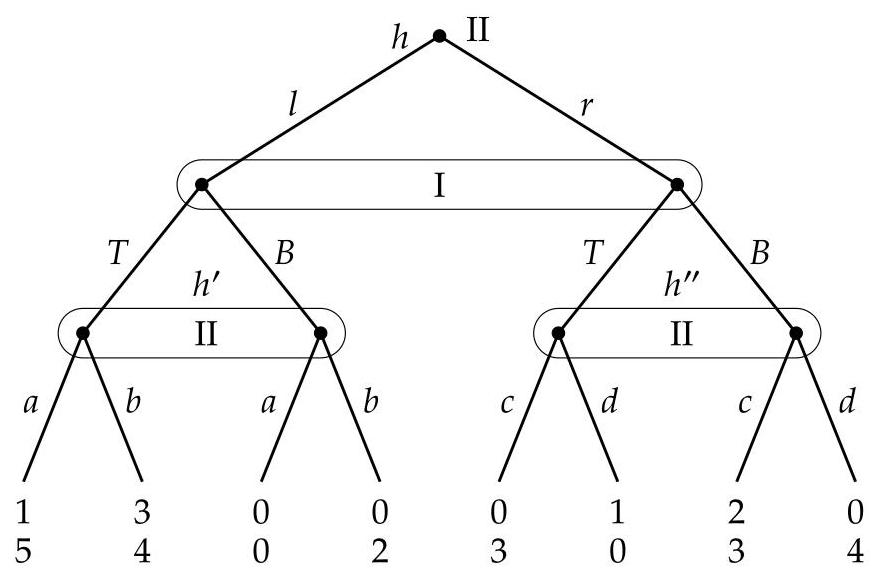
\includegraphics[width=0.6\textwidth]{images/ch10-fig05.jpg}
\caption{参与人$\mathrm{I}$有一个信息集，参与人$\mathrm{II}$有三个信息集 \(h,{h}^{\prime },{h}^{\prime \prime }\) 的扩展型博弈。注意， \(h\) 是一个单元素集，并未在图中明确画出。}
\label{fig:10.5}
\end{figure}

由此引出了精简策略的概念，我们在具有完美信息的博弈树的部分已经接触过这个概念。参与人 \(i\) 的精简策略需要为参与人 \(i\) 的每个信息集指定一个行动，但因那些由于参与人 \(i\) 自己先前的行动（即参与人 \(i\) 的一个行动）而无法到达的信息集除外。书写精简策略时，我们按信息集的固定顺序列出每个信息集的行动；对于那些无法到达的信息集，不指定具体行动，改用特殊符号“*”表示，代表该信息集处可以取任意行动。

在图~\ref{fig:10.5}中，参与人$\mathrm{II}$在选择行动 \(l\) 之后，无法到达信息集 \({h}^{\prime \prime }\)；在选择行动 \(r\) 之后，无法到达信息集\({h}^{\prime }\)。因此，她的精简策略是 \({la}* ,{lb}* ,r*c,r*d\) 。注意，星号代表在考虑完整（未精简）策略时通常会在那个位置的任何未指定行动。所以可以认为参与人$\mathrm{II}$的精简策略 \({la}*\) 同时代表了她的纯策略$lac$和$lad$。

扩展型博弈的精简策略型与它的策略型大体一致，区别仅在于：各参与人只采用约简策略，而非全部纯策略。根据约简策略的构造方式，每个参与人的期望效用都有明确定义，因为未指定的行动不会在博弈过程中对到达博弈树的哪些叶节点有任何影响。图~\ref{fig:10.6}给出了图~\ref{fig:10.5}中博弈的精简策略型。

\begin{figure}[htbp]
\centering
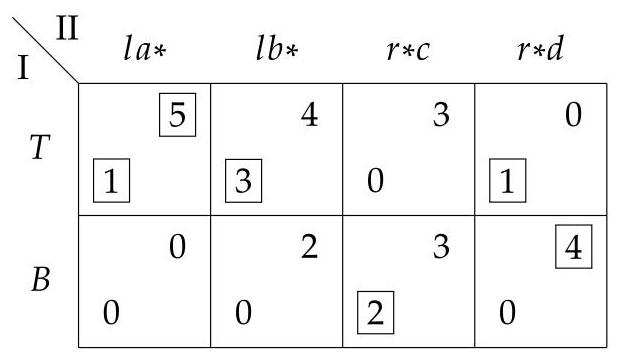
\includegraphics[width=0.4\textwidth]{images/ch10-fig06.jpg}
\caption{图~\ref{fig:10.5}中博弈的精简策略型。在参与人$\mathrm{II}$的策略中，星号“*”表示在由于自己先前的行动而无法到达的信息集上的未指定行动。和前文一样，框中的数字是最优反应收益。}
\label{fig:10.6}
\end{figure}

\section{完美记忆}

图~\ref{fig:10.5}中参与人$\mathrm{II}$的信息集描述了什么？在信息集 \(h\)，参与人$\mathrm{II}$确定自己处于博弈的根节点。在信息集 \({h}^{\prime }\)，她不知道参与人$\mathrm{I}$的行动，但她知道自己之前在根节点做出了行动 \(l\) 。在信息集 \({h}^{\prime \prime }\)，她也不知道参与人 \(\mathrm{I}\) 的行动，但她知道自己之前在根节点做出了行动 \(r\) 。

作为对比，考虑图~\ref{fig:10.7}中的博弈。除了信息集 \({h}^{\prime }\) 和 \({h}^{\prime \prime }\) 合并形成了一个新的包含四个节点的信息集 \({h}^{\prime \prime \prime }\)，它的博弈树和收益与图~\ref{fig:10.5}中的博弈完全相同。此外，为了满足扩展型博弈的定义，信息集 \({h}^{\prime \prime \prime }\) 中的所有节点上的可选行动必须相同；这里将它们称为 \(a\) 和 \(b\)，替换之前在信息集 \({h}^{\prime \prime }\) 处的行动 \(c\) 和 \(d\) 。当参与人$\mathrm{II}$在信息集 \({h}^{\prime \prime \prime }\) 处行动时，她除了知道自己在博弈开始时采取了某个行动，随后是参与人$\mathrm{I}$的行动 \(T\) 或 \(B\)之外，博弈其他的状态一无所知。具体来说，信息集 \({h}^{\prime \prime \prime}\)意味着参与人$\mathrm{II}$已经忘记了自己在根节点所选取的前期行动$l$还是$r$。我们称在图~\ref{fig:10.7}的博弈中，参与人$\mathrm{II}$具有不完美记忆。

非完美回忆会给博弈的解读带来困难，也与我们对理性参与人的基本设定相矛盾。我们后续分析的所有扩展型博弈都具有完美记忆，下面我们给出其{\color{red}正式定义}。例如图~\ref{fig:10.5}展示的就一个具有完美记忆的博弈。在该博弈中，参与人$\mathrm{II}$有两个包含多个节点的信息集 \({h}^{\prime }\) 和 \({h}^{\prime \prime }\)，在这两个信息集上，参与人$\mathrm{II}$都存在信息缺失。我们可以检验这种信息缺失是否源于她自身前期的行动。具体来讲，信息集（以\({h}^{\prime }\)为例）中的每个节点，都可以通过从博弈树的根节点出发的唯一路径到达。沿着这条路径，我们观察到各参与人采取的行动，对于信息集 \({h}^{\prime }\) 的左节点，路径上依次是参与人$\mathrm{II}$的行动 \(l\) 和参与人$\mathrm{I}$的行动 \(T\) ；对于信息集 \({h}^{\prime }\) 的右节点，路径上依次是参与人$\mathrm{II}$的行动 \(l\) 和参与人$\mathrm{I}$的行动行动 \(B\) 。（一般情形下，路径上可能还涉及随机行动。）在这些行动中，我们忽略其他参与人（这里只有参与人$\mathrm{I}$）或随机采取的所有行动。于是我们可以看到，信息集 \({h}^{\prime }\) 中的每个节点之前都有参与人$\mathrm{II}$的行动 \(l\) 。也就是说，信息集中的每个节点对应的自身前期行动序列完全相同。这就是完美记忆的定义。


\begin{definition}
\label{def: 10.1}
在扩展型博弈中，如果对于参与人 \(i\) 的每个信息集 \(h\)，信息集 \(h\) 中的全部节点之前都对应参与人$i$完全相同的自身行动序列，则称参与人 \(i\) 具有完美记忆。如果一个扩展型博弈的所有参与人都具有完美记忆，则称该扩展型博弈具有完美记忆。
\end{definition}

再次强调，完美记忆的核心条件，是参与者$i$的信息集$h$内的所有节点，对应的参与人自身前期行动序列完全一致。我们需要忽略其他参与人的行动，因为倘若博弈中参与人 \(i\) 具有不完美信息，
那对于其他参与人的行动，他一定缺乏部分信息。

\(\Rightarrow\) 务必厘清完美信息和完美记忆之间的区别。这两个概念各自是如何定义的？

\begin{figure}[htbp]
\centering
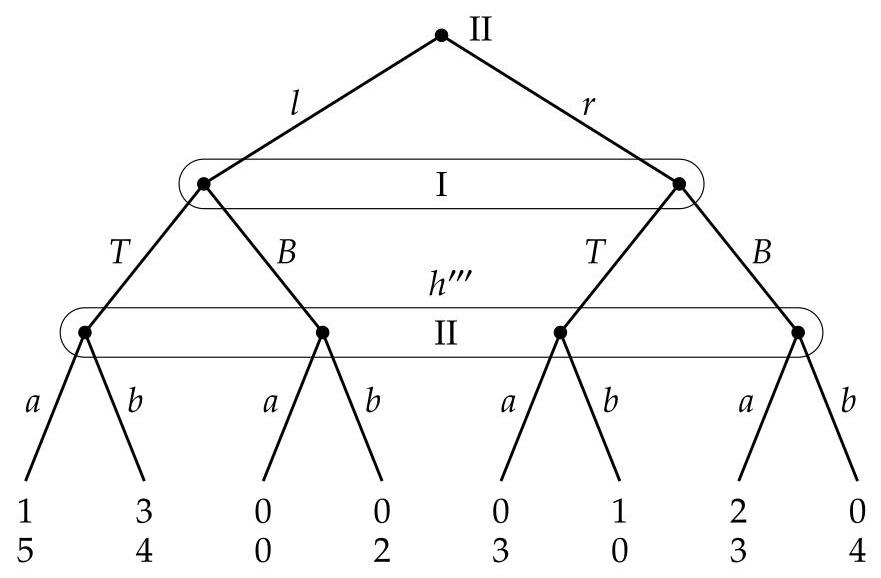
\includegraphics[width=0.6\textwidth]{images/ch10-fig07.jpg}
\caption{参与人$\mathrm{II}$不具备完美记忆的扩展型博弈。}
\label{fig:10.7}
\end{figure}

我们可以验证，图~\ref{fig:10.5}所示的博弈中所有参与人都具备完美记忆。我们已经验证了 \({h}^{\prime }\) 满足定义\ref{def: 10.1}的条件。参与人$\mathrm{II}$另外两个信息集是 \(h\) 和 \({h}^{\prime \prime }\) 。对于 \(h\)，该条件显然成立，因为 \(h\) 仅包含一个节点（由此我们可以直接得到结论：在具有完美信息的博弈中，即信息集为单点集的情况下，所有参与人都具备完美记忆）。对于 \({h}^{\prime \prime }\)， 其中两个节点之前，参与人$\mathrm{II}$的自身行动序列都只有单一行动\(r\)。这表明参与人$\mathrm{II}$具备完美记忆。参与人$\mathrm{I}$只有一个信息集，由于参与人$\mathrm{I}$之前没有采取任何行动，该信息集中的两个节点之前的自身早期行动序列均为空序列。我们通常用 \(\varnothing\) 表示空序列（类似空集）。把空序列也视为一种行动序列是很有帮助的，可以应用定义\ref{def: 10.1}进行判别。

在图~\ref{fig:10.7}中，参与人$\mathrm{II}$不具备完美记忆。原因在于，例如她的信息集 \({h}^{\prime \prime \prime }\)中最左边的节点之前有她自己的早期行动 \(l\)，而最右边的节点之前有行动 \(r\) 。因此，\({h}^{\prime \prime \prime }\)中各个节点所对应的参与人自身前期行动序列并不完全相同。

我们可以借助信息集的含义来理解定义\ref{def: 10.1}。信息集刻画了参与人对博弈状态的认知缺失，即参与人在该时刻并不清楚自己处于信息集中的哪个节点。当所有这些节点的自身早期行动序列相同时，参与人确实无法从已知自己已经采取的行动中获得关于自己在信息集中位置的额外信息（这也符合现实中的正常情形）。另一方面，如果信息集中的某些节点之前有不同的自身早期行动，那么只有当参与人忘记了这些行动时，才会不知道自己在信息集中的位置。出于这个原因，我们称他具有不完美记忆。因此，具有完美记忆的参与人不会有这样的信息集，因为这样的信息集无法如实反映参与人对博弈状态掌握的信息。

然而，定义\ref{def: 10.1}并非关乎博弈的解读。完美记忆是信息集的一种结构性质。只需考察每一个信息集内部的各个节点，检查到达这些节点所对应的参与人自身前期行动序列是否完全一致，即可简便地判断该性质是否成立。整个过程完全不需要对博弈做任何解释。


图~\ref{fig:10.8}展示了一个只有一个参与人的博弈。该参与人有一个包含两个节点的信息集（可选行动包括\(L\) 和 \(R\) ）。两个节点之前的自身早期行动都为\(B\)，由此在这个博弈中参与人$\mathrm{I}$似乎具有完美记忆。然而，如果两个单点信息集的行动名称不同，例如，左边信息集的行动为 \(T\) 和 \(B\)，右边信息集的行动为 \(C\) 和 \(D\) (如图~\ref{fig:10.1}所示)，那么就不再满足完美记忆的条件了。实际上，在图~\ref{fig:10.8}的博弈中参与人$\mathrm{I}$并不具有完美记忆，因原因是不同信息集的行动总是被视为不同的。正式的表述为，只要 \(h \neq  {h}^{\prime }\)，选择集 \({C}_{h}\) 和 \({C}_{{h}^{\prime }}\) 就是不相交的。该假设不失一般性：既可以通过适当地重新命名行动，也可以假设除了博弈树中显示的行动名称外，行动 \(c \in  {C}_{h}\) 的自身标识还包括该行动所在的信息集 \(h\)。

在图~\ref{fig:10.8}的博弈中，参与人$\mathrm{I}$具有不完美记忆的原因在于他忘记了自己先前掌握的信息，也就是随机行动的结果。相比之下，图~\ref{fig:10.7}中的参与人$\mathrm{II}$没有忘记任何先前掌握的信息（她先前知道的所有信息就是她在博弈中率先行动，当她到达信息集 \({h}^{\prime \prime \prime }\) 时，她仍然知道这一点），但她忘记了自己采取的行动。正因如此，有时我们会说，如果一个参与人永远不会忘记她先前知道或做过的事情，那么她就具有完美记忆。定义\ref{def: 10.1}正是对这种说法的精确阐述。

\(\Rightarrow\) 练习~\ref{exer:10.2} 和练习~\ref{exer:10.3} 用于检验读者对完美回忆概念的理解程度。

完美记忆意味着图~\ref{fig:10.3}所示情况不会发生。

\begin{proposition}
\label{pro:10.2}
如果一个参与人具有完美记忆，那么该参与人的一个信息集中的任意两个节点都不会由某条路径相连。
\end{proposition}

\begin{proof}
采用反证法。假设结论不成立，即 \(h\) 是一个具有完美记忆的参与人的信息集，且\(h\)中有两个节点在博弈树中一条路径上，其中一个节点在另一个节点之前。如果有多个这样的节点，令最早的节点为\(u\)（即\(h\)中没有其他节点能够沿着一条路径到达 \(u\)），再取\(h\) 中的另一个节点\(v\)，使得存在一条由 \(u\)通向\(v\) 的路径。（例如，在图~\ref{fig:10.3}中， \(u\) 是博弈树的根节点， \(v\) 是参与人$\mathrm{I}$的信息集中的第二个节点。） 在从 \(u\) 到 \(v\) 的路径上，参与人在决策节点 \(u\) 采取行动 \(c\) 。该行动 \(c\) 先于 \(v\) 。然而，根据 \(u\) 的选取方法，在 \(h\) 中没有其他节点能够通过行动 \(c\)到达\(u\)，也就是说行动\(c\)并不是\(u\)的前期行动。因此，节点\(v\) 和 \(u\) 所对应的该参与者自身前期行动集合是不同的，所以这两个节点的前期自身行动序列肯定也不同。这意味着该参与人具有不完美记忆，与已知条件矛盾。
\end{proof}

\begin{figure}[htbp]
\centering
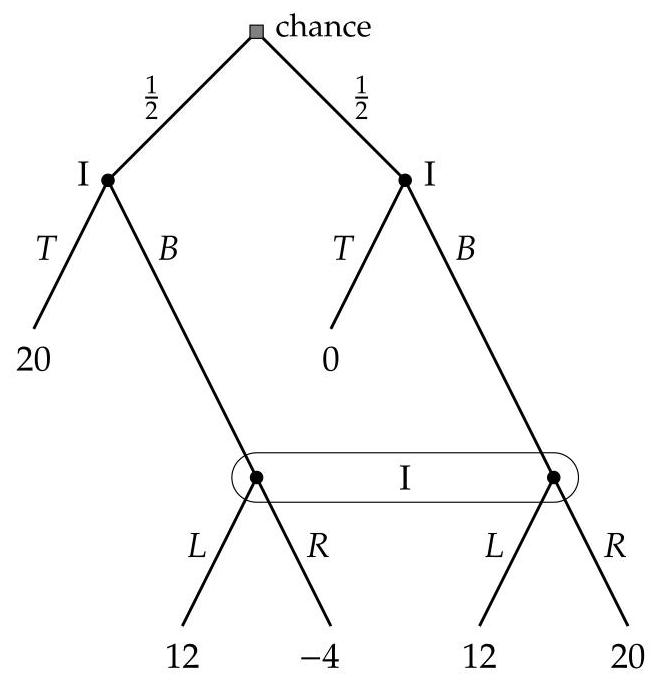
\includegraphics[width=0.5\textwidth]{images/ch10-fig08.jpg}
\caption{参与人$\mathrm{I}$不具有完美记忆的单人博弈。不同信息集的行动通常被视为是不同的，即使它们具有相同的名称（例如，这里的 \(B\) ）。}
\label{fig:10.8}
\end{figure}

图~\ref{fig:10.3}和图~\ref{fig:10.8}中的例子表明，如果单人博弈的信息集包含两个或更多节点，那么该博弈通常不具备完美记忆。

\(\Rightarrow\) 构建一个具有完美记忆的单人博弈，要求并非所有信息集都是单点集。为什么必须引入随机行动？


\section{行为策略}

接下来我们讨论扩展型博弈中的随机化策略。与具有完美信息的博弈（总是存在一个可以通过逆向归纳法找到的纯策略均衡）不同，具有不完美信息的博弈可能需要用到随机策略，图~\ref{fig:10.1}中的例子已经说明了这一点。

\begin{figure}[htbp]
\centering
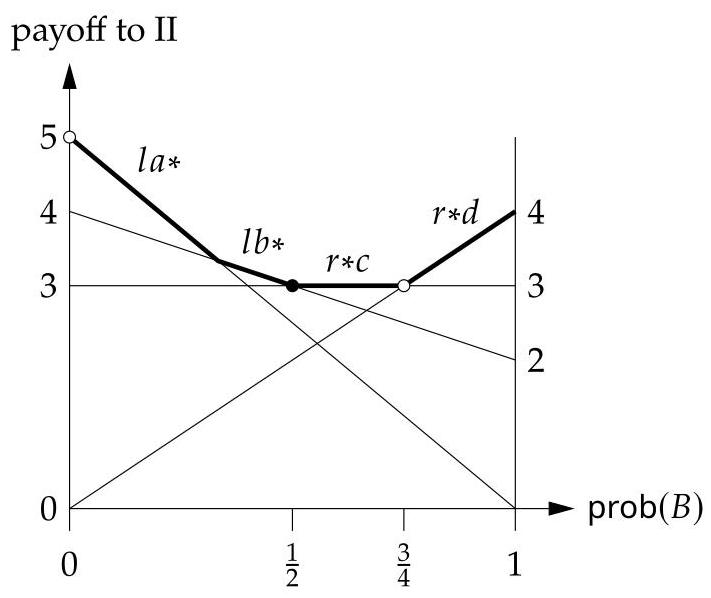
\includegraphics[width=0.5\textwidth]{images/ch10-fig09.jpg}
\caption{图~\ref{fig:10.6}中博弈的参与人$\mathrm{II}$期望效用的上包络。白色和黑色圆点标记了参与人$\mathrm{I}$的均衡策略。}
\label{fig:10.9}
\end{figure}

我们求解图~\ref{fig:10.5}所示博弈的所有均衡，该博弈的精简策略型如图~\ref{fig:10.6}所示。该博弈唯一的纯策略均衡是策略对 \(\left( {T,{la} * }\right)\)。为了找出其余可能存在的混合策略均衡，我们使用上包络法。图~\ref{fig:10.9}展示了参与人$\mathrm{II}$的期望效用，该收益是参与人$\mathrm{I}$选择\(B\)的概率的函数。如图所示，能够令参与者$\mathrm{II}$达到无差异的策略配对仅有三组：当 \(\operatorname{prob}\left( B\right)  = \frac{1}{3}\) 时， \({la} *\) 和 \({lb} *\) ；当 \(\operatorname{prob}\left( B\right)  = \frac{1}{2}\) 时， \({lb} *\) 和 \(r * c\) ；当 \(\operatorname{prob}\left( B\right)  = \frac{3}{4}\) 时， \(r * c\) 和 \(r * d\) 。其中第一组策略组合无法构成均衡，因为面对 \({la} *\) 和 \({lb} *\)，参与人 \(\mathrm{I}\) 的最优反应都是 \(T\)，所以参与人 \(\mathrm{I}\)无法在 \(T\)和\(B\)之间保持无差异，而这是参与人$\mathrm{I}$在均衡中想要在 \(T\) 和 \(B\) 之间进行混合的必要条件。然而，在另外两种情况下，参与人$\mathrm{I}$的纯策略最优反应不同，因此可以构成混合均衡。这些均衡是 \(\left( {\left( {\frac{1}{2},\frac{1}{2}}\right) ,\left( {0,\frac{2}{5},\frac{3}{5},0}\right) }\right)\) 和 \(\left( {\left( {\frac{1}{4},\frac{3}{4}}\right),\left( {0,0,\frac{1}{3},\frac{2}{3}}\right) }\right)\)。

在扩展型博弈中这些混合策略的含义是什么呢？对于参与人 \(\mathrm{I}\)，混合策略 \(\left( {\frac{1}{2},\frac{1}{2}}\right)\) 意味着他以相等的概率选择 \(T\) 和 \(B\) 。对于参与人$\mathrm{II}$，混合策略 \(\left( {0,\frac{2}{5},\frac{3}{5},0}\right)\) 相当于以概率 \(\frac{2}{5}\) 选择 \({lb} *\)，以概率 \(\frac{3}{5}\) 选择 \(r * c\) 。这种混合策略的含义是，每个参与人在博弈开始时就选择一个精简纯策略，该策略是一个在每个可到达的信息集上的行动计划。然后参与人在整个博弈过程中都遵循这个行动计划。具体来说，如果参与人$\mathrm{II}$选择执行 \({lb} *\)，那么她确定地首先会采取行动 \(l\)，然后在她的第二个信息集 \({h}^{\prime }\)采取行动 \(b\)。她的精简纯策略 \(r * c\) 是一个类似的行动计划。

存在一种不同的方式来执行这种混合策略，称为行为策略。行为策略是指在每个信息集上对行动进行随机选择。也就是说，参与人不是在博弈开始时用彩票来确定一个（精简）纯策略，而是每当到达一个信息集时使用一个局部的彩票。在我们的例子中，参与人$\mathrm{II}$的混合策略 \(\left( {0,\frac{2}{5},\frac{3}{5},0}\right)\)按行为策略的执行方式如下：在她的第一个信息集 \(h\)，她分别以概率 \(\frac{2}{5}\) 和 \(\frac{3}{5}\) 采取行动 \(l\) 和 \(r\)。当她到达信息集 \({h}^{\prime }\) 时(只有在她之前采取了行动 \(l\) 时才有可能到达该信息集)，她以概率$0$选择行动 \(a\)，以概率$1$选择行动 \(b\)；在 \({h}^{\prime }\) 处的行为是确定的。类似地，当她到达信息集 \({h}^{\prime \prime }\) 时（之前采取了行动 \(r\)），她确定地选择行动 \(c\)。

\begin{definition}
\label{def:10.3}
在扩展型博弈中，参与人 \(i\) 的行为策略\(\beta\)
是对该参与者的每一个信息集$h$，在其可行行动集合\(C_h\)上定义一个概率分布。对任意\(c \in  {C}_{h}\)，该概率分布由 \(\beta \left( c\right)\) 给出：即每个 \(c \in  {C}_{h}\)，满足\(\beta \left( c\right)  \geq  0\)并且 \(\mathop{\sum }\limits_{{c \in  {C}_{h}}}\beta \left( c\right)  = 1\)。在精简行为策略中，如果无法到达信息集\(h\)（因为在行为策略 \(\beta\) 下，参与人 \(i\) 所有能使其到达 \(h\) 的前期自身行动的概率均为零），则这些概率不做具体规定。
\end{definition}

图~\ref{fig:10.5}中博弈的另一个混合均衡（即参与人$\mathrm{II}$的混合策略 \(\left( {0,0,\frac{1}{3},\frac{2}{3}}\right)\)）可一用来说明精简行为策略的概念。该策略在两种纯策略 \(r * c\) 和 \(r * d\) 之间做随机选择。它也可以作为一种精简行为策略来执行。具体来说，在参与人$\mathrm{II}$的第一个信息集 \(h\) 处，她选择 \(l\) 和 \(r\) 的概率分别为0和1。那么就无法到达信息集 \({h}^{\prime }\)，因为只有当参与人$\mathrm{II}$以正概率选择行动 \(l\) 时才可到达该信息集，而本策略中并不会出现该情况。因此，按照精简行为策略的要求，选择行动 \(a\) 和 \(b\) 的行为概率无需做具体规定。（若要得到一个未精简的行为策略，则需为 \(a\) 和 \(b\) 任意指定一组概率。）在她的信息集 \({h}^{\prime \prime }\) 上，参与人$\mathrm{II}$分别以 \(\frac{1}{3}\) 和 \(\frac{2}{3}\)的概率选择\(c\)和\(d\)。

行为策略的实施当时，是将参与人的随机选择“延后”，直到她到达某个信息集并需要做出下一步行动时，在进行随机选择。不过，参与者也完全可以提前为每一个信息集完成全部随机化，由此得到一套纯策略，并在后续博弈全程执行这套策略。这样行为策略就以混合策略的方式使用。换句话说，行为策略可以被视为特殊的混合策略。

参与人 \(i\) 的行为策略 \(\beta\)，可以通过为该参与人的每个纯策略\(\pi\) 定义一个合适的概率 \(\mu \left( \pi \right)\) 来定义一个混合策略 \(\mu\)，具体构造方式如下：纯策略 \(\pi\) 为每个信息集 \(h \in  {H}_{i}\) 定义了一个行动 \(\pi \left( h\right)\)。当参与人 \(i\) 使用行为策略 \(\beta\) 时，该行动发生的概率为\(\beta \left( {\pi \left( h\right) }\right)\)。由于参与人 \(i\) 在各个信息集 \(h\) 处的这些随机行动是相互独立的，所以纯策略\(\pi\)指定的所有行动都被执行的概率是这些概率的乘积。也就是说，该混合策略的概率为
\begin{equation}
\label{eq:10.3}
\mu \left( \pi \right)  = \mathop{\prod }\limits_{{h \in  {H}_{i}}}\beta \left( {\pi \left( h\right) }\right) .
\end{equation}

我们在将混合策略（例如图~\ref{fig:10.5}中的 \(\mu  = \left( {0,0,\frac{1}{3},\frac{2}{3}}\right)\)）解读为行为策略\(\beta\)时，就已经使用了方式\eqref{eq:10.3}。我们下面将说明，即使像本例这样，混合策略是用精简纯策略的概率来定义的，该式依然成立。行为策略 \(\beta\) 由 \(\beta \left( l\right)  = 0,\beta \left( r\right)  = 1\, \beta \left( c\right)  = \frac{1}{3}\) 和 \(\beta \left( d\right)  = \frac{2}{3}\) 给出，于是有\(\frac{2}{3} = \mu \left( {r * d}\right)  = \beta \left( r\right)  \cdot  \beta \left( *\right)  \cdot  \beta \left( d\right)\) 。该式写成三个行为概率的乘积，分别对应一个信息集；这是因为纯策略需要为每个信息集指定行动，式\eqref{eq:10.3}本身就是对参与人\(i\) 的所有信息集\(h\)去乘积。由于我们考虑的是精简纯策略，项 \(\beta \left( *\right)\) 表示在 \({h}^{\prime }\) 处采取任何行动的行为概率（在里作为精简纯策略 \(r * d\) 的组成部分，这个概率是未明确指定的。显然，该概率等于1。也就是说，当(10.3)应用于精简纯策略 \(\pi\) 时，我们取 \(\beta \left( *\right)  = 1\) 。

容易看出，规定\(\beta \left( *\right)  = 1\)与\eqref{eq:10.3}应用于未精简纯策略是自洽的。例如，考虑未精简的策略型，其中\(r * d\)代表两个纯策略$rad$和$rbd$。将 \(\mu\) 和 \(\beta\) 扩展到未精简的策略形式，这两个纯策略都有获得相应的概率，这里的\(\mu\)正是\(\beta\)所导出的混合策略。无论这些概率是多少（通过将\(r * d\)的概率拆分为$rad$和$rbd$的概率得到），我们都有
\[
\mu \left( {rad}\right)  + \mu \left( {rbd}\right)  = \beta \left( r\right) \beta \left( a\right) \beta \left( d\right)  + \beta \left( r\right) \beta \left( b\right) \beta \left( d\right)  = \beta \left( r\right)  \cdot  \left( {\beta \left( a\right)  + \beta \left( b\right) }\right)  \cdot  \beta \left( d\right) .
\]

在这个等式中，左边是混合策略概率\(\mu \left( {r * d}\right)\)的正确解释，右边是概率 \(\beta \left( r\right)  \cdot  \beta \left( *\right)  \cdot  \beta \left( d\right)\)，这与规定\(\beta \left( *\right)  = \beta \left( a\right)  + \beta \left( b\right)  = 1\)保持一致。

\begin{figure}[htbp]
\centering
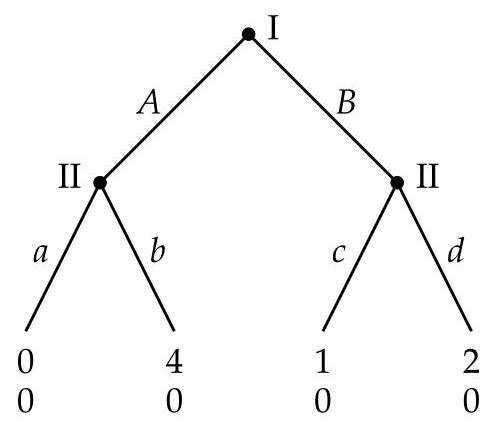
\includegraphics[width=0.3\textwidth]{images/ch10-fig10.jpg}
\caption{参与人$\mathrm{II}$有四个纯策略的博弈。在此博弈中，并非参与人$\mathrm{II}$的所有混合策略都可以表示为行为策略。}
\label{fig:10.10}
\end{figure}

虽然每个行为策略都可以被视为一个混合策略，但反之则不成立。图~\ref{fig:10.10}展示了一个博弈，其中参与人$\mathrm{II}$有四种纯策略 \({ac},{ad},{bc},{bd}\)，这些也是她的精简纯策略。考虑参与人$\mathrm{II}$的混合策略 \(\mu  = \left( {\frac{1}{2},0,0,\frac{1}{2}}\right)\)，她以概率 \(\frac{1}{2}\) 选择纯策略 \({ac}\)，即行动 \(a\) 和 \(c\)，否则选择纯策略 \({bd}\) 。显然，每个行动总体上都有正概率（实际上，每个单独行动发生的概率为 \(\frac{1}{2}\)）。那么，如果\eqref{eq:10.3}成立，每个行动组合也必须有正概率！然而，事实并非如此，因为例如策略$ad$在 \(\mu\) 下的概率为零。原因是当参与人$\mathrm{II}$使用 \(\mu\) 时，行动 \(a\) 和 \(b\) 之间的随机选择与 \(c\) 和 \(d\) 之间的随机选择是相关的。也就是说，知道已经采取了行动 \(a\) 会提供一些关于是否采取了行动 \(c\) 或 \(d\) 的信息（本例中相关性是最大的：选择行动 \(a\) 就意味着选择行动 \(c\) ）。如果这些随机选择是像行为策略所要求的那样，是相互独立的，那么 \(a\) 和 \(b\) 之间的随机选择就不会影响 \(c\) 和 \(d\) 之间的随机选择。

在这个例子中，由 \(\mu\) 刻画的参与人$\mathrm{II}$在图~\ref{fig:10.10}中左信息集处的行为，是以概率 \(\frac{1}{2}\) 选择 \(a\)，以概率 \(\frac{1}{2}\) 选择 \(b\)，行动 \(c\) 和 \(d\) 的选择概率同样各为\(\frac{1}{2}\)。这定义了参与人$\mathrm{II}$的一个行为策略 \(\beta\) 。这个行为策略定义了混合策略\(\left( {\frac{1}{4},\frac{1}{4},\frac{1}{4},\frac{1}{4}}\right)\)，因为它以相等的概率选择每个纯策略。这个混合策略显然与 \(\mu\) 不同。

图~\ref{fig:10.10}的第二个例子是混合策略 \({\mu }^{\prime } = \left( {\frac{1}{6},\frac{1}{3},\frac{1}{4},\frac{1}{4}}\right)\) 。相应的行为策略 \({\beta }^{\prime }\) 的行动概率为 \({\beta }^{\prime }\left( a\right)  = {\beta }^{\prime }\left( b\right)  = \frac{1}{2}\)，因为 \({\beta }^{\prime }\left( a\right)  = {\mu }^{\prime }\left( {ac}\right)  + {\mu }^{\prime }\left( {ad}\right)  = \frac{1}{6} + \frac{1}{3}\) 。类似地， \({\beta }^{\prime }\left( c\right)  = {\mu }^{\prime }\left( {ac}\right)  + {\mu }^{\prime }\left( {bc}\right)  = \frac{1}{6} + \frac{1}{4} = \frac{5}{12}\) 以及\({\beta }^{\prime }\left( d\right)  = {\mu }^{\prime }\left( {ad}\right)  + {\mu }^{\prime }\left( {bd}\right)  = \frac{1}{3} + \frac{1}{4} = \frac{7}{12}\) 。同样，用 \({\beta }^{\prime }\) 对各行动做独立随机化，得到的各纯策略概率与$\mu'$并不一致。例如纯策略\({ac}\)的概率为 \({\beta }^{\prime }\left( a\right)  \cdot  {\beta }^{\prime }\left( c\right)  = \frac{5}{24}\)，该值与\({\mu }^{\prime }\left( {ac}\right)\)并不相等。

在这个例子中，我们所做的是取一个参与人的混合策略 \(\mu\)，并在该参与人的每个信息集上观察由\(\mu\)导出的行为。这种行为定义了某种行为策略\(\beta\)。类似地，\({\beta }^{\prime }\) 是由 \({\mu}^{\prime}\)导出的。该行为策略可能与原始的混合策略不同，原因在于：行为策略中，不同信息集上的随机选择不再相关。但是，给定其他参与人的某些（纯或混合）策略，博弈树上各节点到达概率是不变的。我们说策略 \(\mu\) 和 \(\beta\) 是实现等价的；类似地， \({\mu }^{\prime }\) 和 \({\beta }^{\prime }\) 也是实现等价的。这种实现等价性在任何具有完美记忆的扩展型博弈中都成立，这是下一节讨论的主题。

\section{库恩定理}

信息集由Kuhn(1953)提出的。他在该论文中还定义了完美记忆和行为策略，并证明了这两个概念之间的重要联系。这种联系是扩展型博弈的核心性质，通常被称为“库恩定理”。该定理指出，具有完美记忆的参与人总可以将其混合策略替换为一个与之实现等价的行为策略。

我们为什么要关心参与人是否可以使用行为策略来替代混合策略呢？相比于混合策略，描述行为策略要简洁得多，当博弈规模较大时，这种简化效果尤为显著。例如，考虑一个简化的扑克博弈，每个参与人仅拿到一张牌，这张牌的点数共有13种不同的可能。该博弈的博弈树以一个随机行动开始，参与人 \(\mathrm{I}\) 拿到的牌有 13 种可能性，参与人 \(\mathrm{I}\) 知道自己牌的点数后，可以选择“弃牌”或“加注”。不管博弈的剩余部分如何，仅这部分就已经为参与人\(\mathrm{I}\) 定义了 \({2}^{13} = {8192}\) 种行动组合。假设这些是参与人\(\mathrm{I}\) 的所有纯策略，那么参与人\(\mathrm{I}\) 的混合策略必须指定 8191 个概率（因为概率之和为 1，余下概率由这些概率决定）。相比之下，行为策略会为每张可能的牌指定一个概率（例如弃牌的概率），仅仅是13个不同的数字。因此，行为策略的描述比混合策略要简单得多。

这个例子也让我们直观地理解了为什么行为策略就足够了。参与人\(\mathrm{I}\)在不同决策节点上的行动可以独立地随机化，因为这些节点对应博弈中不相交的情形。没有必要对拿到不同牌的行动设置关联性，因为在任何一局游戏中，只抽取一张牌。

一般来说，参与人会依次做出行动；从先验角度看，将前期行动与后续行动关联起来可能会带来一些好处。这时完美记忆条件就发挥作用了。也就是说，因为完美记忆意味着参与人知道自己所有的前期行动，任何关于前期行动的信息都已经被信息集所包含。所以没有必要将后期行动以前期行动为条件，因为所有前期行动都是参与人已知的。

为了说明这一点，考虑图~\ref{fig:10.7} 中不具有完美记忆的博弈。很容易看出，除了参与人\(\mathrm{II}\) 的纯策略是 \({la},{lb},{ra},{rb}\) 而不是精简策略 \({la} * ,{lb} * ,r * c,r * d\) 之外，这个博弈与图~\ref{fig:10.5} 中的博弈具有相同的策略形式，如图~\ref{fig:10.6} 所示。在这里，参与人\(\mathrm{II}\) 的混合策略 \(\left( {0,\frac{2}{5},\frac{3}{5},0}\right)\)，以概率 \(\frac{2}{5}\) 选择纯策略 \({lb}\)，以概率 \(\frac{3}{5}\) 选择 \({ra}\)，不能表示为行为策略。也就是说，这个行为策略必须分别以概率 \(\frac{2}{5}\) 和 \(\frac{3}{5}\) 选择行动 \(l\) 和 \(r\)，但是行动 \(a\) 和 \(b\) 的概率(分别为 \(\frac{3}{5}\) 和 \(\frac{2}{5}\) )并不独立于早期行动（否则，例如纯策略 \({la}\)）的概率就不会为零)。所以这个属于均衡组成部分的混合策略不能表示为行为策略。使用混合策略为参与人\(\mathrm{II}\)在博弈中提供了更多的行动可能性。

与之相对，图~\ref{fig:10.5}所示的具有完美记忆的博弈中，参与人$\mathrm{II}$的混合策略 \(\left( {0,\frac{2}{5},\frac{3}{5},0}\right)\)表示分别以概率 \(\frac{2}{5}\) 和 \(\frac{3}{5}\) 选择 \({lb} *\) 和 \(r * c\) 。如前所述，这实际上是一种行为策略，之所以可以将行动 \(l\) 与行动 \(b\) 相关联，以及将行动 \(r\) 与行动 \(c\) 相关联，是依靠信息集 \({h}^{\prime }\) 和 \({h}^{\prime \prime }\) 实现的；它们在图~\ref{fig:10.5}中是分开的，但在图~\ref{fig:10.7}中合并成了一个信息集。也就是说，参与人$\mathrm{II}$知道，当她在 \({h}^{\prime }\) 处需要做出行动 \(b\) 时，她清楚记得之前做出了行动 \(l\)；当她在 \({h}^{\prime \prime }\) 处需要做出行动 \(c\) 时，她也清楚记得之前做出了行动 \(r\) 。

在陈述库恩定理之前，我们需要定义一个参与人的两个随机策略\(\mu\)和\(\rho\)实现等价是什么意思。其定义为：如果给定其他参与人的任意策略，当该参与人使用 \(\mu\) 时和使用 \(\rho\) 时，博弈树的每个节点被到达（实现）的概率均相同，那么就称这两个策略是实现等价的。两个实现等价的策略 \(\mu\) 和 \(\rho\) 总是带给每个参与人相同的期望效用，因为无论使用 \(\mu\) 还是 \(\rho\)，到达博弈树的各个叶节点的概率是相同的。

两个策略 \(\mu\) 和 \(\rho\) 在什么时候是实现等价的呢？假设二者都是参与人 \(i\) 的策略。考虑博弈树的一个特定节点，比如 \(u\)。 \(\mu\) 和 \(\rho\) 策略等价意味着，给定其他参与人某一确定策略组合，当参与人 \(i\) 使用\(\mu\)时和使用\(\rho\)时，到达 \(u\) 的概率是相同的。为了到达 \(u\)，博弈必须经过一系列特定的行动序列，包括随机行动，最终走向\(u\)。由于博弈是树结构，所以这个行动序列是唯一的。在这个序列中，一些行动是由随机行动或参与人 \(i\) 之外的其他参与人做出的。因为随机行动的概率和其余参与者的策略都是给定不变的，这部分行动的发生概率也是确定的。通过只考虑其他参与人能够到达\(u\)的固定策略，我们可以假设这些行动的总概率不为零（否则，无论使用 \(\mu\) 还是 \(\rho\)， 到达\(u\) 的概率显然都为零）。因此，比较 \(\mu\) 和 \(\rho\)时，真正重要的是参与人 \(i\) 在通向 \(u\) 的路径上的行动。如果对于每一个节点\(u\)，在 \(\mu\) 和 \(\rho\) 下，参与人 \(i\)在通向\(u\)的路径上自身那一段行动序列的概率都相等，那么 \(\mu\) 和 \(\rho\) 就是实现等价的。这是库恩定理证明过程中的关键点。

\begin{theorem}[Kuhn,1953]
\label{thm:10.4}
如果扩展型博弈中的参与人 \(i\)具有完美记忆，那么对于参与人 \(i\) 的任意混合策略 \(\mu\)，都存在一个与之实现等价的行为策略\(\beta\)。
\end{theorem}

\begin{proof}
我们借助图~\ref{fig:10.11}中的扩展型博弈来演示证明思路，将参与人$\mathrm{II}$作为参与人\(i\)。图中省略了收益；因为只有到达博弈树节点的概率是重要的，收益支付无关紧要。


\begin{figure}[htbp]
\centering
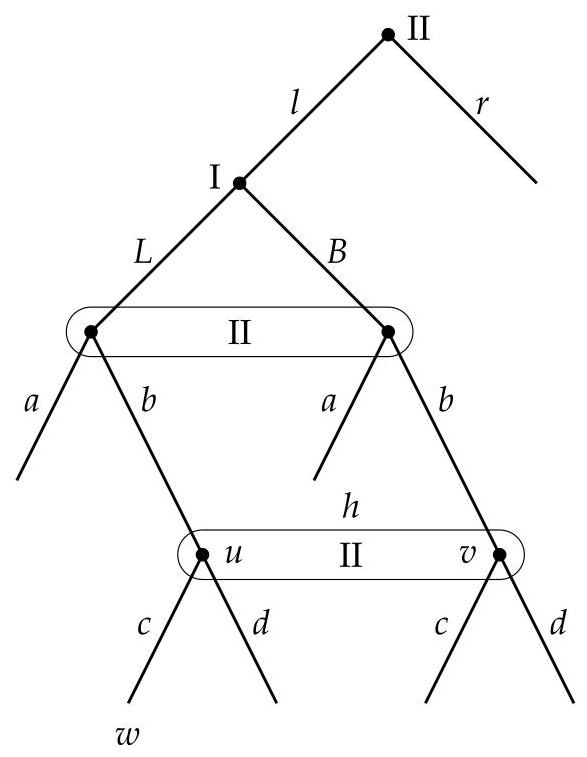
\includegraphics[width=0.4\textwidth]{images/ch10-fig11.jpg}
\caption{该博弈说明了参与人$\mathrm{II}$的行动序列以及库恩定理10.4的证明。支付被省略。}
\label{fig:10.11}
\end{figure}

给定 \(\mu\)，我们想要构建一个实现等价的行为策略 \(\beta\) 。基本思路是，对于参与人 \(i\) 在信息集 \(h\) 处的任何行动 \(c\)，其概率 \(\beta \left( c\right)\)就是参与人 \(i\) 使用 \(\mu\) 时，观察到的选择行动\(c\)的概率。为了得到这个概率，我们考虑参与人 \(i\) 的行动序列。任取博弈树上一个节点\(x\)，取出从根节点走到\(x\)的路径上，所有由参与者\(i\)做出的行动，便得到这样一条行动序列，记为\(\sigma_i(x)\)。例如，如果 \(x\) 是图~\ref{fig:10.11} 中博弈树的叶节点\(w\) 且 \(i = \mathrm{{II}}\)，那么该序列就是 \({\sigma }^{\mathrm{{II}}}\left( w\right)  = {lbc}\)，即依次执行行动 \(l,b,c\)。如果考虑所有参与人，那么到达节点 \(w\) 的行动序列是\({lLbc}\)，该序列包括参与人 \(\mathrm{I}\) 的行动 \(L\)，但在定义\({\sigma }^{\mathrm{{II}}}\left( w\right)\)时会忽略该行动；对于参与人\(\mathrm{I}\)，由\(w\) 定义的自身行动序列只有行动\(L\)，即\({\sigma }^{\mathrm{I}}\left( w\right)  = L\)。

根据定义\ref{def: 10.1}，完美记忆条件表明，对于信息集中的所有节点，参与人自己先前的行动序列是相同的。也就是说，\[h \in  {H}_{i} \Rightarrow  \forall u,v \in  h\;{\sigma }^{i}\left( u\right)  = {\sigma }^{i}\left( v\right) .
\] 图~\ref{fig:10.11} 就给出了一个例子，信息集 \(h\) 中参与人\(\mathrm{II}\) 有两个行动 \(c\) 和 \(d\)，该信息集有两个节点 \(u\) 和 \(v\) 且 \({\sigma }^{i}\left( u\right)  = {\sigma }^{i}\left( v\right)  = {lb}\) 。因此，对于任意\(u \in  h\)，通向\(h\)的行动序列可以唯一地定义为 \({\sigma }_{h} = {\sigma }^{i}\left( u\right)\)，其中\(i\)是在\(h\)处行动的参与人，即\(h \in {H}_{i}\)。此外，我们可以通过\(h\)中的任意行动\(c\)对通向 \(h\)的序列\({\sigma }_{h}\)进行拓展，记作更长的序列\({\sigma }_{h}c\)，读作“\({\sigma }_{h}\)之后接着\({c}\) ”。在本例中，通向\(h\)的序列是 \({\sigma }_{h} = {lb}\)，它可以通过行动 \(c\) 或行动 \(d\) 进行扩展，得到更长的序列 \({lbc}\) 和 \({lbd}\) 。参与人\(i\)的任意行动序列要么是空序列 \(\varnothing\) （例如，如果 \(r\) 是树的根节点，则为 \({\sigma }^{i}\left( r\right)  = \varnothing\) ），要么该序列的最后一步行动$c$是在参与人$i$的某个信息集$h$上做出，因此它可以写成 \({\sigma }_{h}c\)。因此，所有满足\(h \in  {H}_{i}\) 、 \(c \in  {C}_{h}\)的序列\({\sigma }_{h}c\)以及 \(\varnothing\)，构成了参与人 \(i\) 所有可能的行动序列。

现在我们考虑当参与人 \(i\) 使用 \(\mu\) 时，该参与人的某条行动序列\(\sigma\)被执行的概率\(\mu \left\lbrack  \sigma \right\rbrack\) 。该概率\(\mu[\sigma]\)就是在\(\mu\)之下，所有与\(\sigma\)一致的纯策略的概率之和；所谓一致，指这些纯策略规定的行动完全包含\(\sigma\)当中的全部行动。例如，如果图~\ref{fig:10.11}中的 \(\sigma  = {lb}\)，那么与 \(\sigma\) 一致的参与人 \(i\) 的纯策略就是那些指定要执行行动 \(l\) 和 \(b\)的策略，即纯策略 \({lbc}\)和 \({lbd}\)。所以 \begin{equation}
\label{eq:10.4}
\mu \left\lbrack  {lb}\right\rbrack   = \mu \left( {lbc}\right)  + \mu \left( {lbd}\right) ,
\end{equation}其中\(\mu \left( {lbc}\right)\) 和 \(\mu \left( {lbd}\right)\) 分别是纯策略 \({lbc}\) 和 \({lbd}\) 的混合策略概率。

序列 \(\sigma\) 越长，与 \(\sigma\) 一致的纯策略集合就越小。相反，较短的序列有更多与之一致的策略。极端情况是空序列 \(\varnothing\)，因为每个纯策略都与该序列一致。因此，我们有\begin{equation}
\label{eq:10.5}
\mu \left\lbrack  \varnothing \right\rbrack   = 1\text{ . }
\end{equation}

现在我们来看等式\eqref{eq:10.4}的另一种解释。在这个特例中， \({lbc}\)和\({lbd}\)也是行动序列，即带有\({\sigma }_{h} = {lb}\)的\({lbc} = {\sigma }_{h}c\) 和 \({lbd} = {\sigma }_{h}d\) 。所以所有与 \({lbc}\) 一致的纯策略的组合概率 \(\mu \left\lbrack  {lbc}\right\rbrack\) 仅仅是混合策略概率 \(\mu \left( {lbc}\right)\)，同理 \(\mu \left\lbrack  {lbd}\right\rbrack   = \mu \left( {lbd}\right)\)。显然，\(\mu \left\lbrack  {lb}\right\rbrack   = \mu \left\lbrack  {lbc}\right\rbrack   + \mu \left\lbrack  {lbd}\right\rbrack\)。而一般情况，考虑参与人\(i\)的任意信息集\(h\)，我们有下面这个重要等式:\begin{equation}
\label{eq:10.6}
\mu \left\lbrack  {\sigma }_{h}\right\rbrack   = \mathop{\sum }\limits_{{c \in  {C}_{h}}}\mu \left\lbrack  {{\sigma }_{h}c}\right\rbrack  .
\end{equation} 这个等式成立是因为通向\(h\)的序列 \({\sigma }_{h}\)会在 \(h\)处通过某个行动\(c\)得到扩展，从而得到更长的序列 \({\sigma }_{h}c\)。当考虑与这些扩展序列一致的纯策略时，我们得到的刚好是与 \({\sigma }_{h}\)一致的纯策略。

现在我们可以定义与 \(\mu\) 实现等价的行为策略 \(\beta\)。也就是，给定满足\(\mu \left\lbrack  {\sigma }_{h}\right\rbrack   > 0\)的参与人 \(i\) 的信息集 \(h\)，令\begin{equation}
\label{eq:10.7}
\beta \left( c\right)  = \frac{\mu \left\lbrack  {{\sigma }_{h}c}\right\rbrack  }{\mu \left\lbrack  {\sigma }_{h}\right\rbrack  }.
\end{equation} 由\eqref{eq:10.6}可知，上式在\(h\)处的行动集合 \({C}_{h}\)上定义了一个概率分布，这正是行为策略所要求的。在\eqref{eq:10.7}中用到了完美记忆的条件；因为否则，通向信息集 \(h\)的序列\({\sigma }_{h}\)就无法唯一确定。

那\(\mu \left\lbrack  {\sigma }_{h}\right\rbrack   = 0\)的情况呢？这意味着在 \(\mu\) 下，与 \({\sigma }_{h}\) 一致的纯策略的概率为零。换句话说，当参与人 \(i\) 使用 \(\mu\)时，\(h\)是无法到达的。我们很快会证明，对于参与人\(i\)的所有序列 \(\sigma\)，有\(\mu \left\lbrack  \sigma \right\rbrack   = \beta \left\lbrack  \sigma \right\rbrack\)。因此，当参与人使用\(\beta\)时，\(h\)同样无法到达，所以不需要对于 \(c \in  {C}_{h}\)定义 \(\beta \left( c\right)\)，也就是说，根据定义\ref{def:10.3}， \(\beta\)是一个精简的行为策略。或者，我们可以以任意方式定义在\(h\)处的某种行为概率（不过这不会带来任何影响，因为参与人\(i\)不会移动到 \(h\)），例如给 \(h\) 处的每个行动 \(c\) 赋予相等的概率，即令 \(\beta \left( c\right)  = 1/\left| {C}_{h}\right|\) 。

我们声称由\eqref{eq:10.7}定义的\(\beta\)与\(\mu\)是实现等价的。对参与人\(i\)的任意序列\(\sigma\)，我们定义 \(\beta \left\lbrack  \sigma \right\rbrack\)：它是参与人使用 \(\beta\) 时， 执行完\(\sigma\)中全部行动的概率。显然，该概率就是序列内各行动对应概率的乘积。也就是说，如果 \(\sigma  = {c}_{1}{c}_{2}\cdots {c}_{n}\)，那么 \(\beta \left\lbrack  \sigma \right\rbrack   = \beta \left( {c}_{1}\right) \beta \left( {c}_{2}\right) \cdots \beta \left( {c}_{n}\right)\)。当 \(n = 0\) 时 \(\sigma\)是空序列 \(\varnothing\)，在这种情况下我们设置 \(\beta \left\lbrack  \varnothing \right\rbrack = 1\) 。结合\eqref{eq:10.7}，我们得到
\[
\beta \left\lbrack  {{c}_{1}{c}_{2}\cdots {c}_{n}}\right\rbrack   = \beta \left( {c}_{1}\right) \beta \left( {c}_{2}\right) \cdots \beta \left( {c}_{n}\right)  = \frac{\mu \left\lbrack  {c}_{1}\right\rbrack  }{\mu \left\lbrack  0\right\rbrack  }\frac{\mu \left\lbrack  {{c}_{1}{c}_{2}}\right\rbrack  }{\mu \left\lbrack  {c}_{1}\right\rbrack  }\cdots \frac{\mu \left\lbrack  {{c}_{1}{c}_{2}\cdots {c}_{n - 1}{c}_{n}}\right\rbrack  }{\mu \left\lbrack  {{c}_{1}{c}_{2}\cdots {c}_{n - 1}}\right\rbrack  } = \mu \left\lbrack  {{c}_{1}{c}_{2}\cdots {c}_{n}}\right\rbrack
\]结合\eqref{eq:10.5}，所有中间项都抵消了。（结合图~\ref{fig:10.11} 中像 \(\sigma  = {lbc} = {c}_{1}{c}_{2}{c}_{3}\) 这样的例子理解这一点最为直观。）由于对于参与人 \(i\) 的所有序列\(\sigma\)都有 \(\beta \left\lbrack  \sigma \right\rbrack   = \mu \left\lbrack  \sigma \right\rbrack\)，根据定理\ref{thm:10.4}之前的阐释，策略\(\beta\)和\(\mu\)是实现等价的；原因在于：博弈树上任意节点$u$，都是由所有参与人和机会的唯一行动序列到达的。其他参与人的行动概率是固定的，所以真正起作用的是参与人 \(i\) 的行动序列\({\sigma }^{i}\left( u\right)\)，无论参与人 \(i\) 使用 \(\beta\) 还是 \(\mu\)，该序列发生的概率都是相同的。\end{proof}

把上面这套证明过程，对定义\ref{def:10.3}之后的例子或上面的图~\ref{fig:10.10}再推演一遍是有启发性的；同时也可以借此练习，学会在小规模博弈当中求解行为策略。

\section{蒙提霍尔问题的行为策略}

我们通过博弈论框架下的非标准版本的蒙提·霍尔问题(Monty Hall problem)，来阐释行为策略这一概念。最初的版本源自一档早期电视竞猜节目的概率谜题，节目主持人名为蒙提·霍尔。参赛者从三扇关闭的门当中选择一扇，来赢得奖品。其中一扇门后面是奖品（一辆汽车），另外两扇门后面是参赛者不想要的东西（一只山羊）。一旦参赛者选择了其中一扇门，蒙提·霍尔会打开剩下两扇门中的一扇，露出一只山羊，然后给参赛者一个机会，让其选择换到另一扇未打开的门。问题是，她应该换门吗？参赛者现在面临着两个选项（最初选择的门和另一扇未打开的门），二者中奖概率似乎均等，所以换门似乎没有意义。然而，正确的答案是，参赛者最初选择正确门的概率 \(\frac{1}{3}\)，并不会因为蒙提·霍尔打开另一扇门露出山羊的行为而改变，因为蒙提·霍尔知道奖品在哪里，他永远都能选出一扇藏有山羊的门来打开。因此最初选择的门中奖概率概率仍然是 \(\frac{1}{3}\)，另一扇未打开的门后面有奖品的概率是 \(\frac{2}{3}\)，因此参赛者确实应该换门。

这种分析与许多人的直觉相悖，他们认为，主持人打开一扇藏有山羊的门，反倒是印证了自己一开始就选对了门（该想法是错误的）。此外，他们怀疑蒙提·霍尔只是试图诱使他们放弃正确的选择。如果蒙提·霍尔只是有时打开另一扇有山羊的门并提供换门的机会，那么这种怀疑是正确的。很明显，如果蒙提·霍尔只在参赛者选择了正确的门时才提供换门机会，那么换门就意味着她会失去奖品，因此她永远不应该换门。简而言之，蒙提·霍尔问题的原始版本的标准答案仅在蒙提·霍尔总是提供换门机会这一前提下才成立。

\begin{figure}[htbp]
\centering
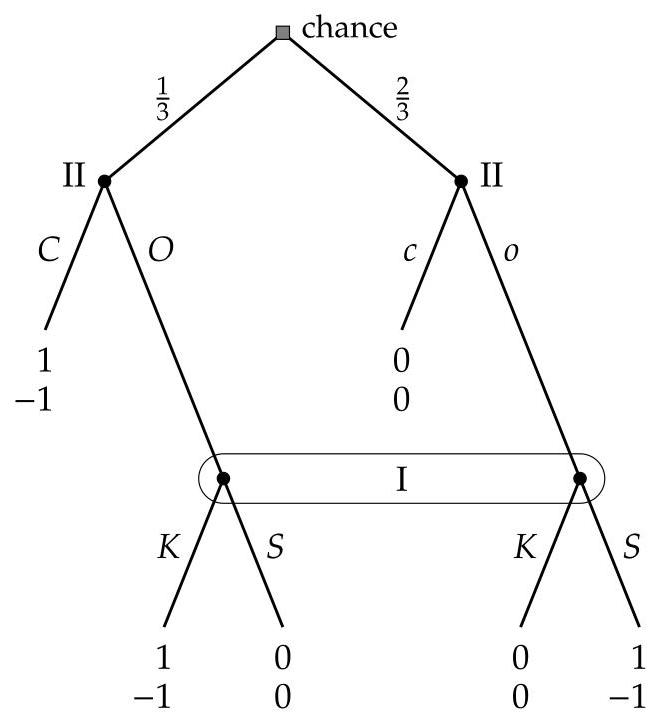
\includegraphics[width=0.5\textwidth]{images/ch10-fig12.jpg}
\caption{我们将（修改版本的）蒙提·霍尔问题视为参与人$\mathrm{I}$（参赛者）和参与人$\mathrm{II}$（电视节目主持人蒙提·霍尔）之间的博弈。参赛者选择正确门的概率为 \(\frac{1}{3}\) （左侧的随机行动），蒙提·霍尔可以选择保持门关闭（行动 \(C\) 和 \(c\) ），或者打开另一扇没有奖品的门（行动 \(O\) 和 \(o\)）。一旦主持人打开一扇门，参与人$\mathrm{I}$可以保持她最初的选择（$K$）或换到剩下的未打开的门（$S$）。收益为$1$意味着参与人$\mathrm{I}$获得奖品，该收益由参与人$\mathrm{II}$支付；收益为0则代表参赛者没有获得奖品。}
\label{fig:10.12}
\end{figure}

图~\ref{fig:10.12}展示了一个新的博弈：参与人$\mathrm{I}$是参赛者，参与人$\mathrm{II}$是蒙提·霍尔。在参赛者选择了三扇门中的一扇后，蒙提·霍尔有多种选择。我们假定奖品等概率藏在任意一扇门的后方。蒙提·霍尔知道参赛者是否选择了正确的门，这一点体现在他的两个决策节点上。左节点有两个行动 \(C\) 和 \(O\)，右节点有两个行动 \(c\) 和 \(o\)，他可以在两个节点上独立地做出选择。行动 \(C\)和\(c\)代表蒙提保持门关闭，行动\(O\)和\(o\)代表他打开另一扇后面有山羊的门。在这种情况下，参赛者（不知道自己是否选择了正确的门）可以坚持自己的选择（$K$）或换到另一扇未打开的门（$S$），然后参赛者要么获得奖品，要么一无所获。我们假设主办电视台倾向于避免送出奖品，因此这是一个零和博弈。

该博弈与本章图~\ref{fig:10.1}中的介绍性博弈具有相同的结构，只是两位参与人的角色互换，并且收益和随机概率不同。它具有以下策略型:


\begin{figure}[H]
\begin{center}
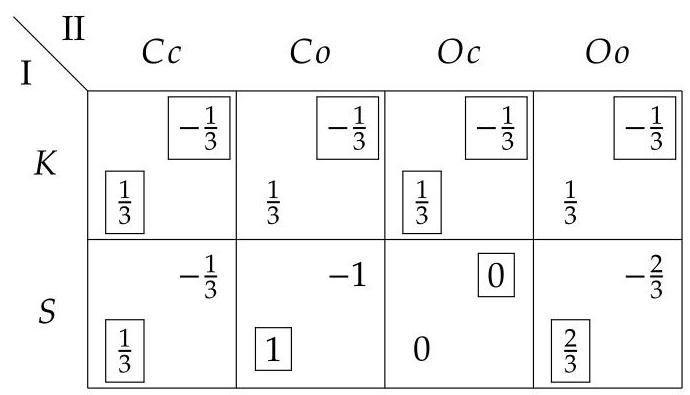
\includegraphics[width=0.5\textwidth]{images/ch10-fig13.jpg}
\end{center}
\hspace*{3em}
\label{fig:10.8}
\end{figure}

尽管这个博弈是零和博弈，但我们还是展示了两个参与人的期望效用，这样更容易看出最优反应。如果参赛者选择\(K\)，即矩阵{\color{red}(10.8)}中的第一行，那么她的期望效用恒等于\(\frac{1}{3}\)，参与人$\mathrm{II}$的所有纯策略都是最优反应。因此，这是一个退化博弈。当蒙提·霍尔从不打开门（策略 \({Cc}\)）时，参赛者同样会得到收益 \(\frac{1}{3}\)，此时她甚至没有换门的机会。因此，\(K\) 和 \({Cc}\) 互为最优反应，构成纯策略均衡$(K，Cc)$，博弈的值为\(\frac{1}{3}\)。

我们现在研究两位参与人的所有均衡策略集合。第二个纯策略均衡是 $(K, Oc)$，即蒙提·霍尔仅在参赛者首次选择了正确的门时才打开另一扇门（也就是前文所说的“试图诱使她换门”）。在这个均衡中，针对\({Oc}\)，参赛者的唯一最优反应是\(K\)。因此，根据零和博弈的命题\ref{prop:8.3}，参与人\(\mathrm{I}\)唯一极大极小策略（也是所有均衡当中参赛者必选的策略）就是\(K\)。

另一方面，参与人\(\mathrm{II}\) 有许多均衡策略，因为他的所有纯策略都是对\(K\)的最优反应，甚至策略\({Co}\)和\({Oo}\)在混合均衡中都可能有正概率。其中一种这样的混合策略是 \(y = \left( {0,0,\frac{1}{2},\frac{1}{2}}\right)\)，即分别以概率 \(\frac{1}{2}\) 采用 \({Oc}\) 和 \({Oo}\) 。那么，第一行\(K\)给参与人\(\mathrm{II}\)的期望效用恒为\(- \frac{1}{3}\)；第二行\(S\)的期望效用也是 \(- \frac{1}{3}\)，所以就主持人自己的收益而言，\(y\)也是参与人\(\mathrm{II}\) 的一个极大极小策略。另一个极大极小策略是 \({y}^{\prime } = \left( {0,\frac{1}{3},\frac{2}{3},0}\right)\)，该策略具备同样的性质。按照\({y}^{\prime }\)，蒙提·霍尔以概率 \(\frac{1}{3}\)采用策略\({Co}\)，即只有当参赛者最初选错门时才向她提出换门，这一提议看起来很奇怪，因为只要参赛者换门肯定就能获得奖品；然而，\({y}^{\prime }\)也以概率 \(\frac{2}{3}\) 选择与之相反的策略 \({Oc}\) 。混合策略$y$以\(\frac{1}{2}\)概率选用的纯策略$Oo$，正是原始的蒙提·霍尔问题里主持人永远打开另一扇后面有山羊的门的策略；倘若参赛者选择$S$，该策略下参赛者可以获得\(\frac{2}{3}\)的收益。即便如此，在本博弈中参赛者绝不应当换门：只要以任意正概率选择换门，就不再是极大极小策略（面对策略$Oc$时，换门带来的收益会低于\(\frac{1}{3}\)）。


可以证明，在这个博弈中，参与人\(\mathrm{II}\)的所有最优混合策略都是上述极大极小策略\({Cc},{Oc},y\)以及\({y}^{\prime }\)的凸组合。除了\({y}^{\prime }\)之外，这些都是行为策略。作为纯策略，\({Cc}\) 和 \({Co}\) 显然是行为策略。采用策略 \(y\) 时，参与人\(\mathrm{II}\)的行为是在左决策节点始终选择 \(O\)，在右决策节点以\(\frac{1}{2}\)的概率在\(c\) 和 \(o\) 之间随机选择。策略 \({y}^{\prime }\) 不是行为策略，下表给出该策略在行动组合\({Cc},{Co},{Oc},{Oo}\)上的分布:

\begin{center}
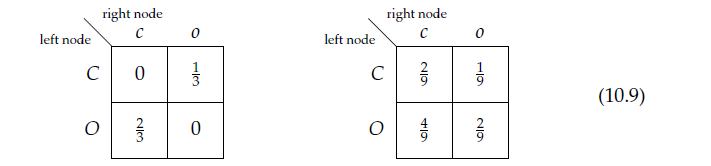
\includegraphics[width=0.9\textwidth]{images/ch10-fig15.png}
\end{center}
\hspace*{3em} 

{\color{red}(10.9)}中的右表给出了行为策略\({\beta }^{\prime}\)，根据库恩定理，它与混合策略 \({y}^{\prime }\)是实现等价的。该行为策略以概率 \(\frac{1}{3}\) 和 \(\frac{2}{3}\) 在 \(C\) 和 \(O\) 之间进行随机选择，以概率 \(\frac{2}{3}\) 和 \(\frac{1}{3}\) 在 \(c\) 和 \(o\) 之间进行随机选择。将行为策略\({\beta}^{\prime}\)还原为纯策略上\({Cc},{Co},{Oc},{Oo}\)的概率分布，是混合策略\(\left( {\frac{2}{9},\frac{1}{9},\frac{4}{9},\frac{2}{9}}\right)\)，该混合策略为选择\(S\)的参与人\(\mathrm{II}\)带来的期望效用为\(- \frac{1}{3}\)。

图~\ref{fig:10.13} 从几何角度展示了参与人\(\mathrm{II}\) 的这些极大极小策略。左图展示了混合策略单纯形，右图展示了代表行为策略概率对的正方形。令\(p\) 是主持人选择\(O\)的概率（正方形的纵坐标，方向向下），\(q\)是他选择\(o\)的概率（横坐标），那么他的四种纯策略 \({Cc},{Co},{Oc},{Oo}\) 被选择的概率分别为\(\left( {1 - p}\right) \left( {1 - q}\right),\left( {1 - p}\right) q,p\left( {1 - q}\right)\) 和 \({pq}\) 。取\(p,q \in  \left\{  {\frac{1}{4},\frac{1}{2},\frac{3}{4}}\right\}\)，可以定义一组网格线，两幅图中均画出了该网格。但作为混合策略单纯形的一个子集，这个网格是“扭曲”且非凸的，这是因为行为策略的凸组合是一般的混合策略，通常不是行为策略。而右侧的正方形是凸的，作为该正方形子集的极大极小行为策略集也是凸的。行为策略\({\beta }^{\prime }\)就属于该集合，并且是 \({Cc}\)和\(y\)的凸组合。


\begin{figure}[htbp]
\centering
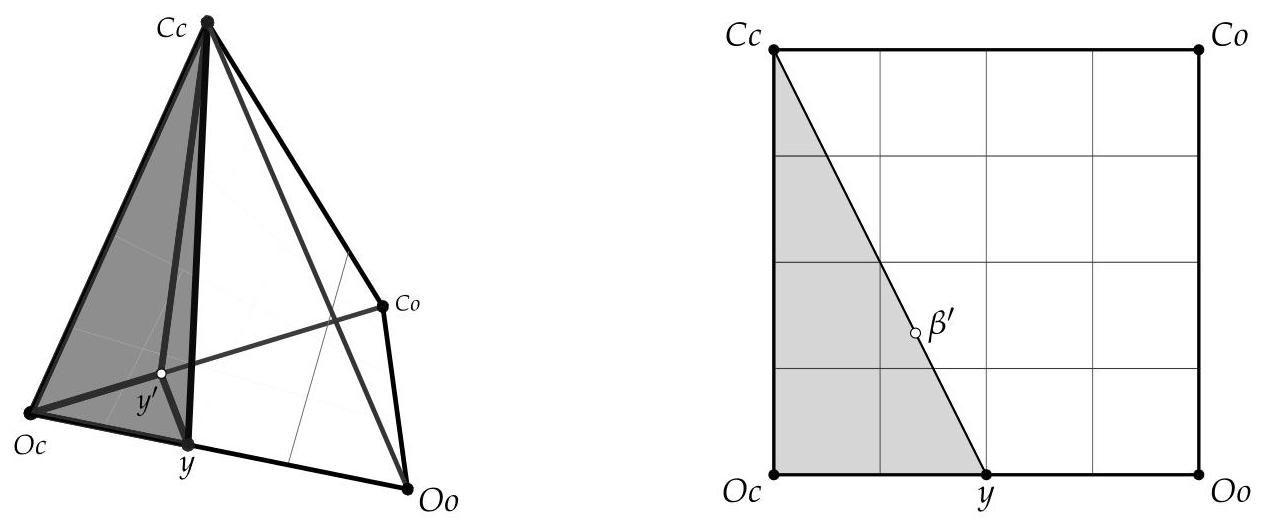
\includegraphics[width=0.9\textwidth]{images/ch10-fig14.jpg}
\caption{左图：博弈 (10.8) 中（参与人\(\mathrm{II}的\)）的混合策略单纯形，灰色部分是极大极小策略子集，它的顶点为 \({Cc},{Oc},y,{y}^{\prime }\) 的。“扭曲的网格”展示了行动概率为 \(\frac{1}{4}\)倍数的行为策略。右图：图~\ref{fig:10.12}中扩展型博弈的行为策略正方形。图中标出了与\({y}^{\prime }\) 实现等价的行为策略\({\beta }^{\prime }\)，并且绘制了相同的网格。阴影三角形是极大极小行为策略集。}
\label{fig:10.13}
\end{figure}

纯策略是正方形的四个角点（与 {\color{red}(10.9)}内单元格位置一一对应），它们也是混合策略单纯形的顶点。

\section{子博弈与子博弈完美均衡}

第\ref{chp: 具有完美信息的博弈树}章讨论的具有完美信息的扩展型博弈中，子博弈是博弈树的任意子树：选取博弈树上某一节点作为子树的根节点，该节点及其全部后继节点就构成子树。在考虑具有不完美信息的博弈时，这个定义需要加以修正，每个参与人都必须知道他们已经进入了子树。

\begin{definition}
在扩展型博弈中，子博弈是博弈树满足下列条件的任意子树：每个信息集要么是子树节点的子集，要么与子树节点不相交。
\end{definition}

换句话说，如果任意信息集 \(h\) 包含子树的某个节点，那么 \(h\) 必须完全包含在子树中。这意味着在 \(h\) 处行动的参与人知道他或她处于子博弈中。不需要考虑与该子树不存在任何共有节点的那些信息集，因为它们和子树互不相交。

在图~\ref{fig:10.14} 中，以参与人\(\mathrm{I}\) 的决策节点为根的子树定义了该博弈的一个子博弈。与之相反，参与人\(\mathrm{II}\) 的第二个信息集中的一个节点不是子博弈的根节点。以图中参与人 \(\mathrm{I}\) 选择行动 \(B\) 之后的节点为例：这个信息集既不包含在以该节点为根的子树中，也不与该子树互不相交。

\begin{figure}[htbp]
\centering
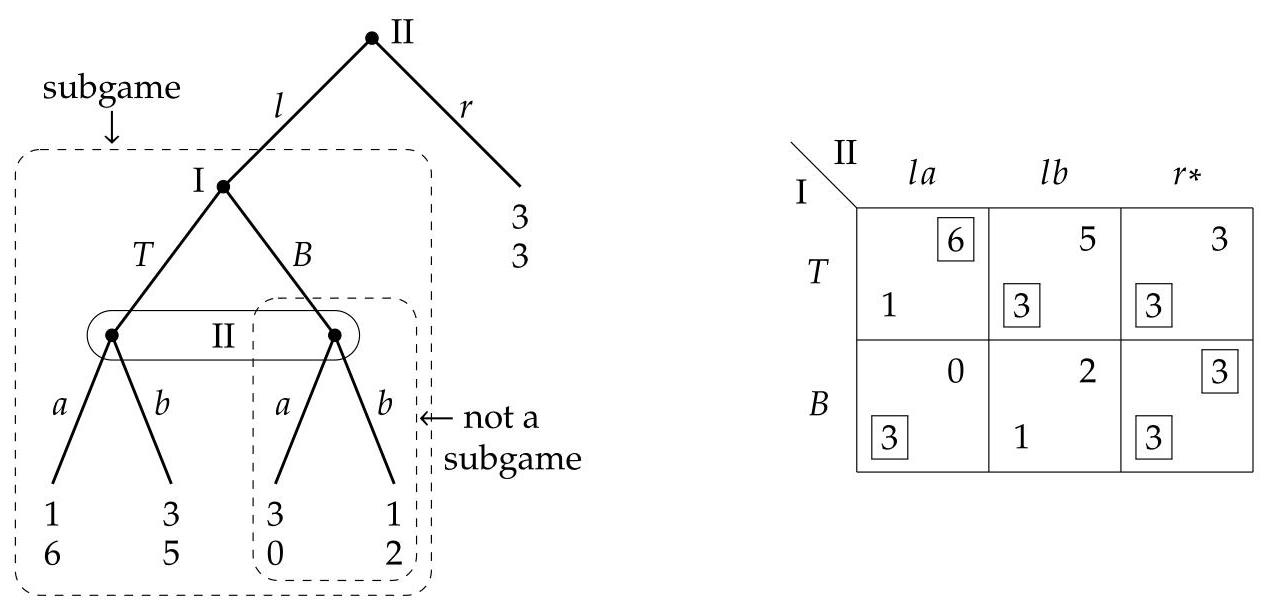
\includegraphics[width=1.0\textwidth]{images/ch10-fig16.jpg}
\caption{扩展型博弈及其子博弈，以及该博弈的精简策略型。该博弈只有一个均衡是子博弈完美均衡，参见图~\ref{fig:10.15}。}
\label{fig:10.14}
\end{figure}

一个博弈的平凡子博弈是博弈本身，或者是博弈树的任意叶节点。有些博弈没有其他子博弈，例如图~\ref{fig:10.1}或图~\ref{fig:10.5}中的博弈。

如果每个参与人都有完美记忆，那么根据定理\ref{thm:10.4}（Kuhn Theorem），任何混合策略都可以被一个实现等价的行为策略替代。因此，任何均衡中的策略都可以假定为是行为策略。对于行为策略，只需忽略与子博弈不相交的信息集的行为概率，可以很容易地将其限制在子博弈中。对于混合策略组合来说，要定义策略在子博弈上的限制就要困难得多。

\begin{definition}
在具有完美记忆的扩展型博弈中，子博弈完美均衡是一个行为策略组合，它在博弈的每个子博弈上都构成均衡。
\end{definition}

图~\ref{fig:10.14}右侧是左侧扩展型博弈的精简策略型。图~\ref{fig:10.15}展示了从参与人$\mathrm{I}$行动开始的非平凡子博弈及其策略型。这个子博弈有一个唯一的混合均衡，其中参与人$\mathrm{I}$以概率 \(\frac{2}{3},\frac{1}{3}\) 选择 \(T,B\)，参与人$\mathrm{II}$以概率 \(\frac{1}{2},\frac{1}{2}\) 选择 \(a,b\) 。参与人$\mathrm{I}$和II的最终收益分别为2和4，用这些收益替代子博弈，可以得到一个较小的博弈，其中参与人$\mathrm{II}$在 \(l\) 和 \(r\) 之间进行选择。

这个较小的博弈显示在图~\ref{fig:10.15}的右侧。因为这个小博弈具有完美信息，通过逆向归纳法可以找到一个子博弈完美均衡。通过逆向归纳法可知，参与人$\mathrm{II}$肯定会选择 \(l\) 。在最终的整体行为策略中，参与人$\mathrm{I}$以概率 \(\frac{2}{3},\frac{1}{3}\) 混合 \(T,B\)，参与人$\mathrm{II}$肯定会选择 \(l\)，并以概率 \(\frac{1}{2},\frac{1}{2}\) 混合 \(a,b\) 。这个行为策略组合是一个子博弈完美均衡。

\begin{figure}[htbp]
\centering
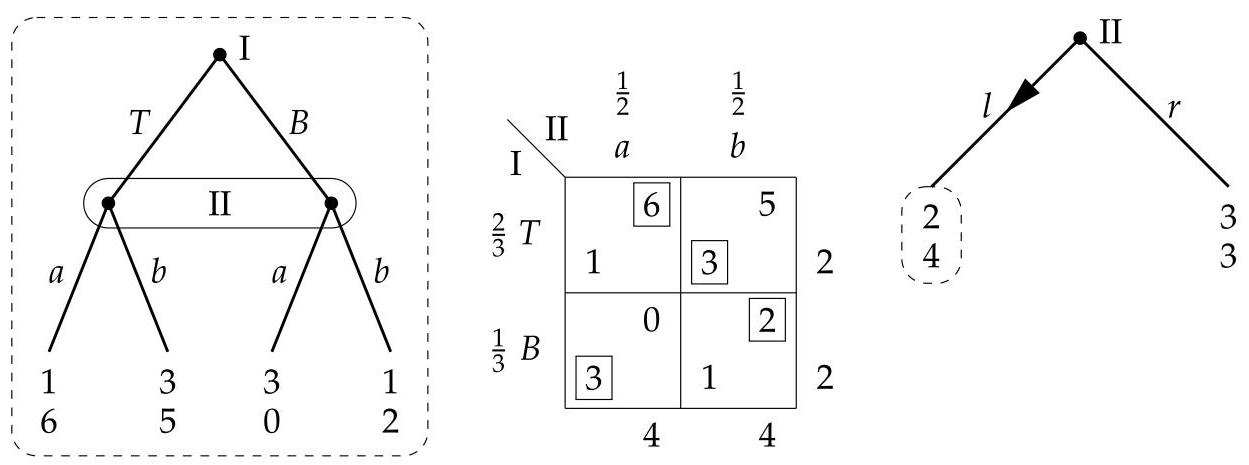
\includegraphics[width=0.9\textwidth]{images/ch10-fig17.jpg}
\caption{图~\ref{fig:10.14}中博弈的子博弈，以及其唯一的混合均衡，收益为2和4。在整个博弈中，如图右侧所示，子博弈被这些收益所替代，因此参与人$\mathrm{II}$在根节点的最优行动是 \(l\) 。这定义了子博弈完美均衡。}
\label{fig:10.15}
\end{figure}

计算子博弈的均衡并用得到的均衡收益替代子博弈这一步骤，是对具有完美信息博弈中的逆向归纳步骤的推广。在具有完美信息的博弈中，这个逆向归纳步骤相当于在一个非常简单的子博弈中找到单个参与人的最优行动，在这个子博弈中每个行动都直接导向一组收益；该最优行动在该子博弈中构成一个均衡。在具有不完美信息的博弈中，子博弈可能涉及多个参与人，求解均衡通常更困难。

图~\ref{fig:10.10}中扩展型博弈的上述子博弈完美均衡，是精简策略型的混合策略均衡 \(\left( {\left( {\frac{2}{3},\frac{1}{3}}\right) ,\left( {\frac{1}{2},\frac{1}{2},0}\right) }\right)\)，它也定义了一对行为策略。另一个均衡是精简纯策略对 \(\left( {B,r * }\right)\) 。策略 \(r *\) 只是参与人$\mathrm{II}$的一个精简行为策略，因为它没有指定她在第二个信息集(当她采取行动 \(r\) 时该信息集无法到达)的行动 \(a\) 和 \(b\) 的概率。但这个均衡不是子博弈完美均衡，因为我们已经求出了该博弈中唯一的子博弈完美均衡。

一般来说，与完全信息博弈的情形相同，只有当每个参与人的行为策略（或纯策略）不是精简精简，而是完整定义的，即为参与人的每个信息集定义了一个概率分布（或确定性行动）时，扩展型博弈的一个均衡才能被称为子博弈完美均衡。

我们已经结合图~\ref{fig:10.14}中的例子介绍了如何找到子博弈完美均衡，该方法是对逆向归纳法的推广。我们将在下面定理的证明中对该方法进行一般性阐述。

\begin{theorem}
任何具有完美记忆的扩展型博弈都存在由行为策略构成的子博弈完美均衡。
\end{theorem}

\begin{proof} 如果博弈树仅由一个节点组成，该节点同时是博弈树的根节点和唯一的叶节点，并标注有每个参与人的收益，那么该定理显然成立。因为每个参与人只有一个策略（什么都不做），该策略组合构成博弈的均衡，并且这个均衡显然也是子博弈完美均衡。

因此，假设博弈树不仅仅由一个节点组成。我们通过归纳法求解该博弈的子博弈完美均衡，步骤如下。首先，找到该博弈的一个以\(u\)为根节点的子博弈：该子博弈不仅仅是一个叶节点，并且它自身不再含有非平凡子博弈。这样的子博弈是存在的：因为如果整个博弈的根节点不满足这个条件，那么考虑一个以\(u\)为根节点的非平凡子博弈，然后继续这样操作，直到找到一个内部不再包含其他子博弈的子博弈。

第二步，考虑这个子博弈的一个均衡。根据定理\ref{theo:6.5} (Nash,1951)，该均衡一定存在；再由定理\ref{thm:10.4} (Kuhn,1953)，该均衡可以表示为行为策略。由于这个子博弈自身没有子博弈，这个均衡是该子博弈的一个子博弈完美均衡。在整个博弈中，用一个叶节点替换该子博弈的根节点\(u\)，该叶节点的收益是子博弈完美均衡中的期望收益。这样得到的博弈树的节点数就会减少，因此可以重复上述操作，直到 \(u\) 是原博弈的根节点。然后将得到的行为策略组合起来，就为原博弈定义一个行为策略组合。根据构造过程可知，这个策略组合是子博弈完美均衡。 \end{proof}

\begin{figure}[htbp]
\centering
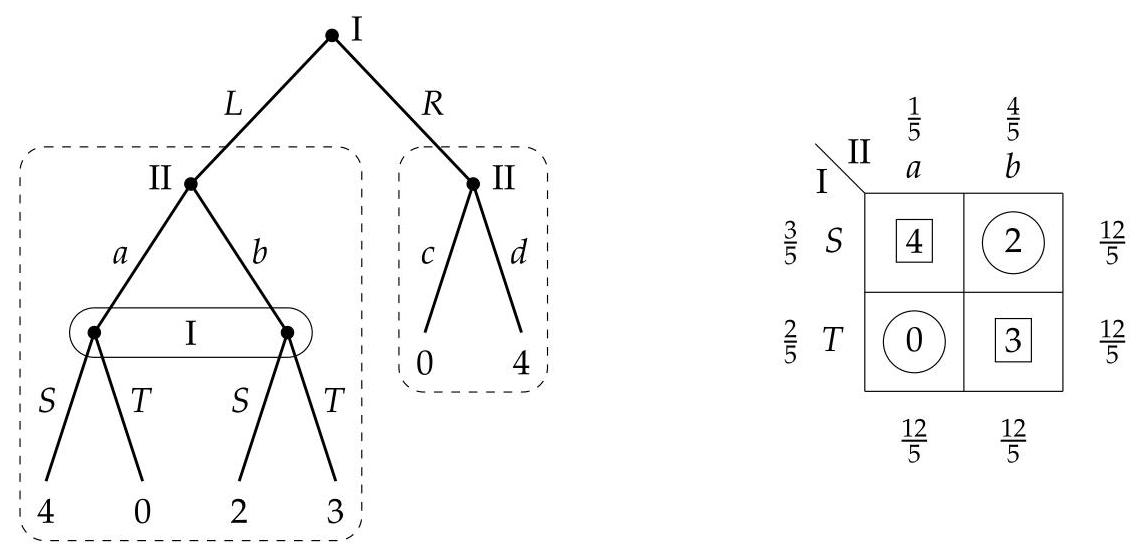
\includegraphics[width=0.9\textwidth]{images/ch10-fig18.jpg}
\caption{左:零和博弈，显示参与人$\mathrm{I}$的收益，以及它的非平凡子博弈。右:左子博弈的策略形式，以及它的最优混合策略。}
\label{fig:10.16}
\end{figure}

我们以图~\ref{fig:10.16}中的例子来演示子博弈的用法，这是一个零和博弈；给出的收益是参与人$\mathrm{I}$的收益。该博弈有两个非平凡子博弈，每个子博弈都以参与人$\mathrm{II}$的行动开始。在右侧的子博弈中，子博弈完美均衡下，作为最小化方的参与人$\mathrm{II}$显然会选择行动\(c\)，此时参与人$\mathrm{II}$的收益为0。左子博弈是一个 \(2 \times  2\) 博弈，其策略形式如图~\ref{fig:10.16}右侧所示。这个博弈有一个唯一的混合均衡，使用“差分技巧”求得均衡为 \(\left( {\left( {\frac{3}{5},\frac{2}{5}}\right) ,\left( {\frac{1}{5},\frac{4}{5}}\right) }\right)\)，参与人$\mathrm{I}$的收益为 \(\frac{12}{5} = {2.4}\)，参与人$\mathrm{II}$的收益为 -2.4。它刻画了参与人在左侧子博弈中的最优行为，并且是整个博弈行为策略的一部分。在博弈树的根节点，参与人$\mathrm{I}$会选择 \(L\)，因为这会给他带来更高的收益2.4，由于该博弈是零和博弈，该数值就是博弈唯一的值。

即使不构建策略型，也可以仅通过分析博弈树而来找到这个博弈的所有均衡，包括那些不是子博弈完美的均衡。由于该博弈是零和博弈，在任意均衡中，每个参与人的收益都等于他的极大极小收益，因此参与人$\mathrm{I}$的收益是2.4，参与人$\mathrm{II}$的收益是 -2.4。如果以正概率选择 \(R\)，那么作为最小化方的参与人$\mathrm{II}$必须选择 \(c\)，否则她的期望效用会更低。如果参与人$\mathrm{II}$选择 \(c\)，与选择 \(L\) 然后采用上述混合 \(S\) 和 \(T\) 的极大极小策略相比，这会降低参与人$\mathrm{I}$的收益。因此，在任何均衡中参与人$\mathrm{I}$一定会选择 \(L\)，其行为策略与前面给出的保持一致。然而，这意味着参与人$\mathrm{II}$永远不会被到达她的右决策节点，参与人$\mathrm{II}$可以在 \(c\) 和 \(d\) 之间进行随机化，只要参与人$\mathrm{I}$的期望效用不超过2.4，也就是满足 \(\operatorname{prob}\left( d\right)  \leq  {0.6}\) 。参与人$\mathrm{II}$在右节点的这一类行为，加上上述以概率\(\frac{1}{5},\frac{4}{5}\)随机选择\(a,b\)的行为，就构成了该博弈任意均衡中参与人$\mathrm{II}$的行为策略集。

\section{延伸阅读}

10.2节中软件公司之间竞争的例子改编自Turocy and von Stengel(2002)。

信息集由Harold Kuhn (1953)提出。Kuhn将实现等价策略简称为“等价”策略。在他的定义17中指出，如果对于参与人 \(i\) 的每个纯策略 \(\pi\)，以及参与人 \(i\) 的每个在采用 \(\pi\) 策略时可达（“相关”）的信息集 \(h\)，在采用 \(\pi\) 策略时， \(h\) 中的所有节点都是可达（“可能发生”）的，那么参与人 \(i\) 具有完美记忆。该定义与本书给出的完美回忆定义\ref{def: 10.1}是等价的；本书的定义改编自Selten (1975, 27页)。


精简行为策略的概念并非标准概念，但本书在此引入它，是因为它与行为策略的对应关系，恰如精简纯策略与纯策略的对应关系。

其他关于不完美信息扩展型博弈，其他教材也有相关论述，可参见Osborne and Rubinstein (1994, 11章) 以及Gibbons (1992, 第2章第4节)。

我们对定理\ref{thm:10.4}(Kuhn Theorem)的证明基于行动序列。这些序列在von Stengel(1996)提出的序列型中起着核心作用。序列型是一种策略层面的描述方式：它不考虑纯策略，而是考虑序列\(\sigma\)，这些序列以概率\(\mu \left\lbrack  \sigma \right\rbrack\)被采用，且对于所有 \(h \in  {H}_{i}\) 满足式\eqref{eq:10.6}与式\eqref{eq:10.5}。策略型的规模可能是扩展式博弈规模的指数倍，而序列型与原博弈树的规模相当。例如，可以借助与博弈树规模相同的线性规划，就可以求解零和博弈。

蒙提·霍尔问题由Selvin (1975)提出。Friedman (1998)对其行为假设进行了讨论和检验。尽管我们的博弈论分析表明，当蒙提·霍尔并非总是提供换门选项时，不换门是非常合理的选择，但这仍然被视为一种“选择异常”。

\section{第 10 章习题}

\begin{exercise}\label{exer:10.1}
把一个 \(m\times n\) 双矩阵博弈表示为扩展式博弈，有两种方式：参与人\(\mathrm{I}\) 先行动或参与人\(\mathrm{II}\)。请解释这两种构造方式，举例会有助于说明。两种构造下，每位参与人各有多少个决策节点？博弈树的终止节点数量是多少？此处为什么需要引入信息集？
\end{exercise}

\begin{exercise}\label{exer:10.2}
以下哪些扩展型博弈具有完美记忆？如果不具有完美记忆，原因是什么？对于每个具有完美记忆的扩展型博弈，找出其所有混合策略均衡（包括纯策略均衡）。
\end{exercise}

\begin{center}
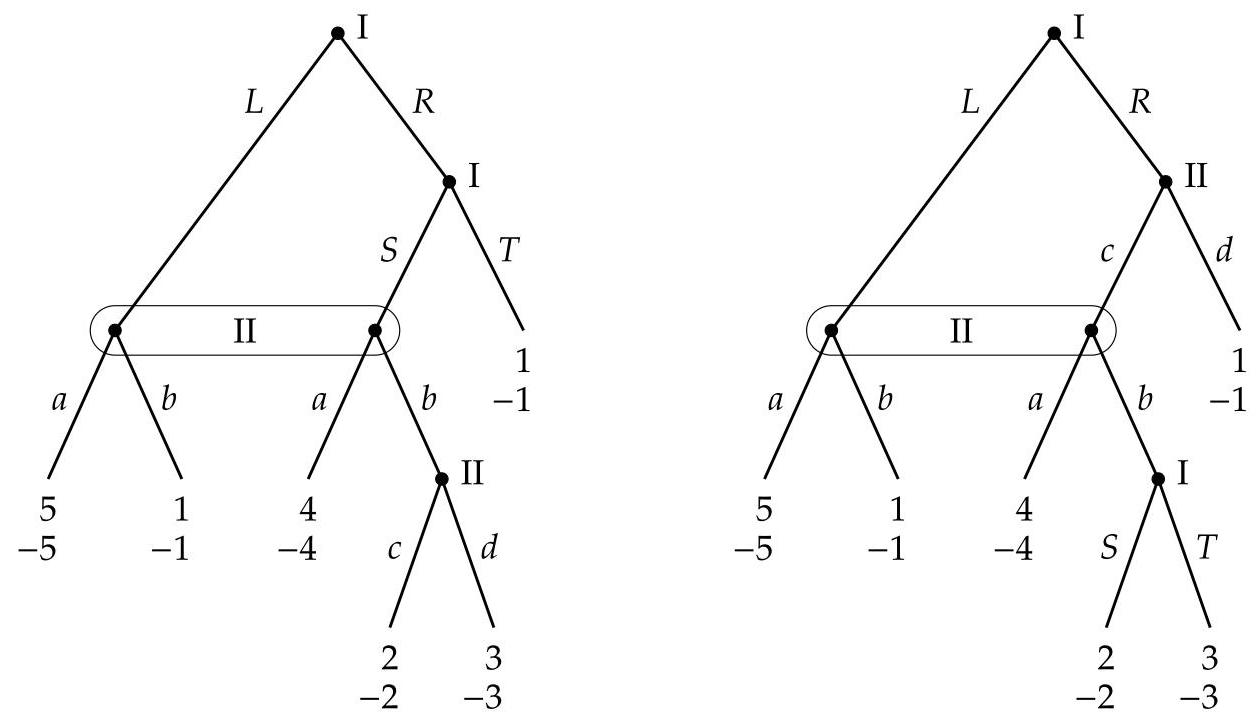
\includegraphics[width=0.9\textwidth]{images/ch10-fig19.jpg}
\end{center}
\hspace*{3em} 

\begin{exercise}\label{exer:10.3}
以下哪些扩展型博弈具有完美记忆？如果不具有完美记忆，原因是什么？对于每个具有完美记忆的扩展型博弈，找出其所有混合策略均衡（包括纯策略均衡）。
\end{exercise}

\begin{center}
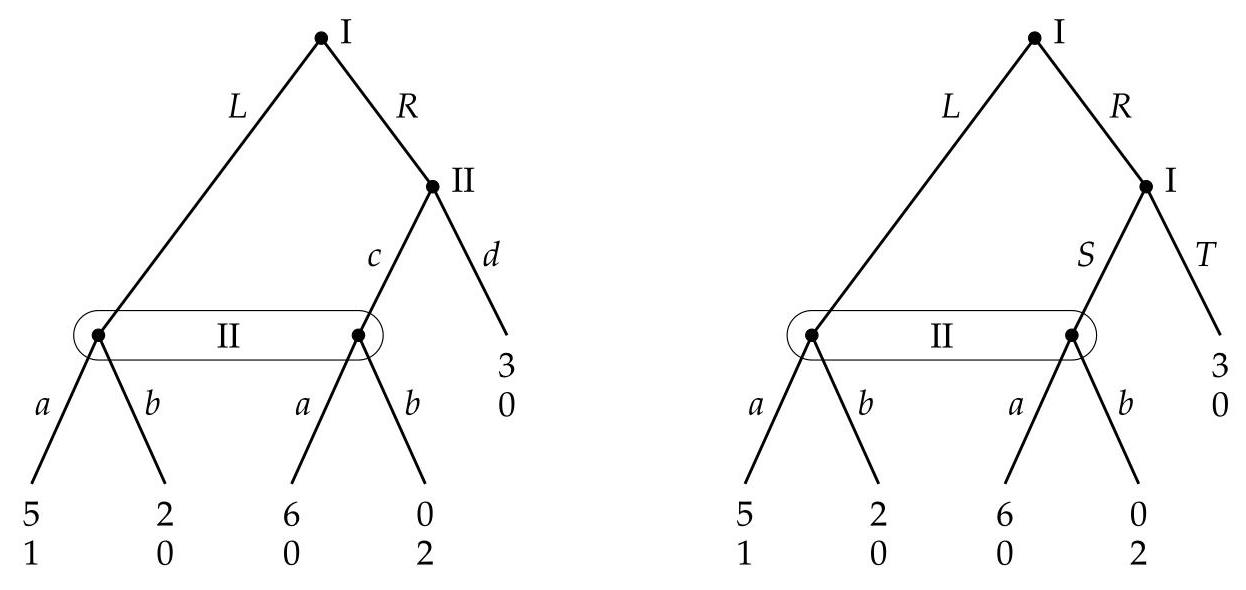
\includegraphics[width=0.9\textwidth]{images/ch10-fig20.jpg}
\end{center}
\hspace*{3em} 

\begin{exercise}\label{exer:10.4}
考虑以下零和博弈，这是一个改编自Kuhn(1950)的简化版扑克游戏。一副牌有三张牌(高、中、低等级)，每个参与人发一张牌。所有发牌情况的可能性相同，当然参与人拿到的牌不同。参与人不知道对方拿到的牌。参与人\(\mathrm{I}\) 看到自己的牌后，有加注(R)或弃牌(F)的选项。当他弃牌时，他输给参与人\(\mathrm{II}\) 一个单位。当他加注时，参与人\(\mathrm{II}\) 有跟注(m)或弃牌(p)的选项。当参与人\(\mathrm{II}\) 选择“弃牌”时，她要付给参与人\(\mathrm{I}\) 一个单位。当参与人\(\mathrm{II}\) 选择“跟注”时，牌面大的参与人获胜，牌面小的参与人要付给获胜参与人两个单位。

(a) 绘制一个具有信息集的扩展型博弈来模拟这个游戏，并在叶节点标注参与人\(\mathrm{I}\) 的收益。

(b) 对该博弈做化简：假定在某个信息集上，无论其他参与者的行动或是随机行动过去和将来如何，参与者的某一个行动总是不差于另一个行动，则参与者会选择该行动。画出化简之后的扩展型博弈。

(c) 请问 (b) 中的简化与弱被占优策略有什么关系？为什么这里的简化是合理的？

(d) 给出 (b) 中简化后游戏的策略形式，并找出该游戏的一个均衡。在该均衡中，各参与人的行为策略概率是多少？均衡时各参与人的唯一收益是多少？
\end{exercise}

\begin{exercise}\label{exer:10.5}
对于一个具有完美记忆的扩展型博弈，证明任意子博弈的根节点（起始节点）所在的信息集一定是单元素集（即只包含该节点）。[提示:使用命题\ref{pro:10.2}。]
\end{exercise}

\begin{exercise}\label{exer:10.6}
找出这个扩展型博弈的所有纯策略或混合策略均衡。其中哪些是子博弈完美均衡？
\end{exercise}

\begin{center}
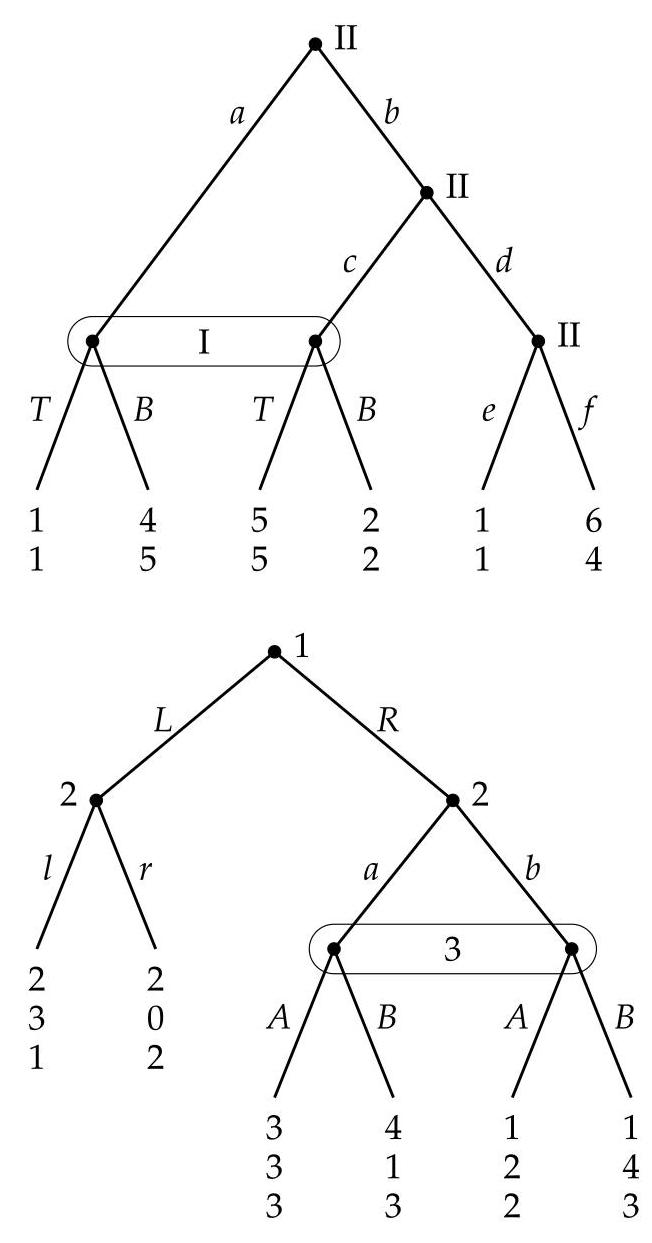
\includegraphics[width=0.5\textwidth]{images/ch10-fig21.jpg}
\end{center}


\begin{exercise}\label{exer:10.7}
考虑这个三人扩展型博弈。在终端节点处，顶部、中部和底部的收益分别属于参与人1、2、3。求解全部混合策略意义下的子博弈完美均衡。
\end{exercise}

\begin{figure}[H]
\begin{center}
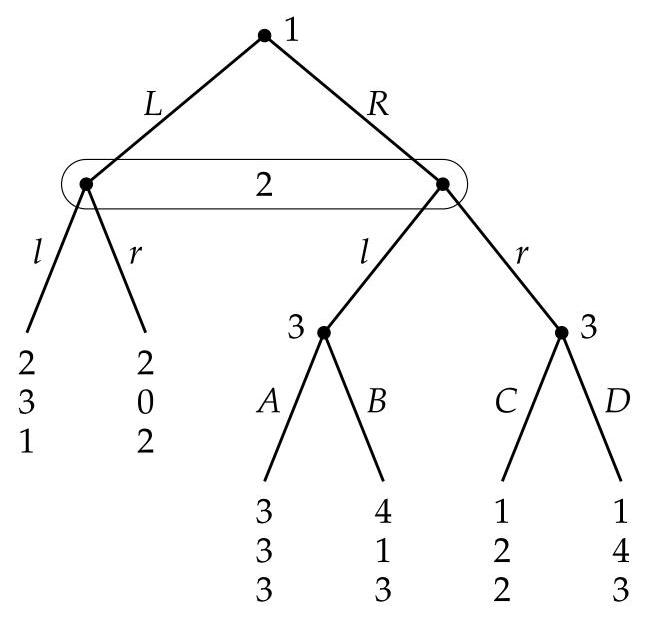
\includegraphics[width=0.5\textwidth]{images/ch10-fig22.jpg}
\end{center}
\end{figure}


\begin{exercise}\label{exer:10.8}
考虑这个三人扩展型博弈。求解全部混合策略意义下的子博弈完美均衡。
\end{exercise}